\documentclass[compress]{beamer}
\usepackage{ifthen,verbatim}

\newcommand{\isnote}{}
\xdefinecolor{lightyellow}{rgb}{1.,1.,0.25}
\xdefinecolor{darkblue}{rgb}{0.1,0.1,0.7}

%% Uncomment this to get annotations
%% \def\notes{\addtocounter{page}{-1}
%%            \renewcommand{\isnote}{*}
%% 	   \beamertemplateshadingbackground{lightyellow}{white}
%%            \begin{frame}
%%            \frametitle{Notes for the previous page (page \insertpagenumber)}
%%            \itemize}
%% \def\endnotes{\enditemize
%% 	      \end{frame}
%%               \beamertemplateshadingbackground{white}{white}
%%               \renewcommand{\isnote}{}}

%% Uncomment this to not get annotations
\def\notes{\comment}
\def\endnotes{\endcomment}

\setbeamertemplate{navigation symbols}{}
\setbeamertemplate{headline}{\mbox{ } \hfill
\begin{minipage}{5.5 cm}
\vspace{-0.75 cm} \small
\end{minipage} \hfill
\begin{minipage}{4.5 cm}
\vspace{-0.75 cm} \small
\begin{flushright}
\ifthenelse{\equal{\insertpagenumber}{1}}{}{Jim Pivarski \hspace{0.2 cm} \insertpagenumber\isnote/\pageref{numpages}}
\end{flushright}
\end{minipage}\mbox{\hspace{0.2 cm}}\includegraphics[height=1 cm]{../cmslogo} \hspace{0.1 cm} \includegraphics[height=1 cm]{../tamulogo} \hspace{0.01 cm} \vspace{-1.05 cm}}

\newcommand{\s}[1]{{\mbox{\scriptsize #1}}}

\begin{document}
\begin{frame}
\vfill
\begin{center}
\textcolor{darkblue}{\Large $Z' \to \mu\mu$ and Alignment/Misalignment}

\vfill
\begin{columns}
\column{0.3\linewidth}
\begin{center}
\large
Jim Pivarski
\end{center}
\end{columns}

\begin{columns}
\column{0.3\linewidth}
\begin{center}
\scriptsize
{\it Texas A\&M University}
\end{center}
\end{columns}

\vfill
27 August, 2010

\end{center}
\end{frame}

%% \begin{notes}
%% \item This is the annotated version of my talk.
%% \item If you want the version that I am presenting, download the one
%% labeled ``slides'' on Indico (or just ignore these yellow pages).
%% \item The annotated version is provided for extra detail and a written
%% record of comments that I intend to make orally.
%% \item Yellow notes refer to the content on the {\it previous} page.
%% \item All other slides are identical for the two versions.
%% \end{notes}

\small

\begin{frame}
\frametitle{State of alignment in brief: data}
\begin{itemize}
\item Tracker Alignment
\begin{itemize}
\item basic procedures have been mature since CRAFT
\item studying weak modes through vertex constraints, invariant mass
  constraints, and comparison of collisions to cosmics
\item discovered 10's of $\mu$m bows/kinks in sensors; adding
  non-rigid alignment parameters to fit them
\end{itemize}

\item Muon Alignment
\begin{itemize}
\item relative tracker/muon position established with track-based
  method, in good agreement with survey measurements
\item track-based and hardware DT alignments are producing similar
  results: largest discrepancy is a 4~mm twist from one end of the
  barrel with respect to the other (13~m apart)

\vspace{0.1 cm}
\hspace{0.5 cm}hardware barrel geometry used in offline reprocessing

\vspace{0.1 cm}
\item CSC alignment pieced together from beam-halo tracks, hardware
  disk-bending measurements, and tracks from the tracker to find the
  disks: mostly orthogonal measurements
\end{itemize}
\end{itemize}
%% \hspace{-0.83 cm} \textcolor{darkblue}{\Large Outline2}
\end{frame}

\begin{frame}
\frametitle{State of alignment in brief: MC}
\begin{itemize}
\item 50~pb$^{-1}$ scenario:
\begin{itemize}
\item tracker: randomly misaligned by throwing Gaussian deviates
\item muon: simulated cosmic-ray followed by collisions alignment using real algorithms on Monte Carlo samples
\end{itemize}

\item STARTUP used in current MC productions:
\begin{itemize}
\item tracker: simulated cosmic-ray alignment using real algorithms
\item muon: simulated cosmic-ray alignment using real algorithms
\item \textcolor{darkblue}{weakly constrained modes in the real alignment are weakly
  constrained in this Monte Carlo scenario, {\it but won't necessarily drift in the same direction with the same magnitude}}
\end{itemize}

\item Tracker weak mode scenarios:
\begin{itemize}
\item nine systematic distortions of an ideal tracker for studying the
  effects of potential weak modes on analyses
\end{itemize}
\end{itemize}

\href{https://twiki.cern.ch/twiki/bin/view/CMS/SWGuideAlignmentConstants}{\tt \scriptsize \textcolor{blue}{https://twiki.cern.ch/twiki/bin/view/CMS/SWGuideAlignmentConstants}}
\end{frame}

\begin{frame}
\frametitle{Context: how to use the scenarios}
\begin{itemize}
\item IDEAL geometry is too optimistic, but a well-defined state of
  the system: resolution can't get any better than this
\item STARTUP is a rough guide for how bad the geometry could be
\begin{itemize}
\item uncertainties in geometry are primarily systematic
\item if we could identify the shape and magnitude of the errors, we
  would correct them in the real-data geometry
\item okay for planning analyses: ``statistical reach with
  misalignment is $X$,'' but not for doing analyses ``we compared
  IDEAL and STARTUP, so our uncertainty from alignment is $X$''
  (unless $X$ is sub-dominant)
\end{itemize}
\item An analysis driven by misalignment uncertainties may need to do
  tests with special geometries, produced using the latest information
  from alignment studies (example in this talk)
\end{itemize}
\end{frame}

\begin{frame}
\frametitle{Context: important distinctions}
\begin{itemize}
\item \textcolor{darkblue}{Smearing (``high multipole moments''):} some
  misalignment uncertainties are tightly localized; in any reasonable
  binning of physics quantities, their effect merely broadens the
  distribution
\begin{itemize}
\item can be modeled in a misalignment scenario because patches of
  $\eta$, $\phi$ space form a statistical ensemble
\item examples: statistical errors, bows and kinks of tracker sensors,
  CSC chamber position uncertainties derived from comparison with
  photogrammetry
\end{itemize}

\item \textcolor{darkblue}{Skewing (``low multipole moments''):} others are
  uncertainties about large-scale twists or stretching of the system
  (tracker and muon); this biases distributions or smears them in a way
  that depends on kinematics
\begin{itemize}
\item similar to ``cosmic variance'' in cosmology: only one sky
\item examples: $Z$-expansion and other weak modes of the tracker,
  twist uncertainty of muon barrel from the single comparison between
  track-based and hardware alignments
\end{itemize}
\end{itemize}
\end{frame}

\begin{frame}
\frametitle{Example: muon barrel twist}
\begin{itemize}
\item Tracker alignment procedure is purely track-based, but in the
  muon system we have track-based (TB) and hardware (HW)

\item The two methods independently ``found'' the muon chambers

\vspace{0.1 cm}
Diagram shows differences between geometries as exaggerated displacements in a wheel end-view:

\vfill
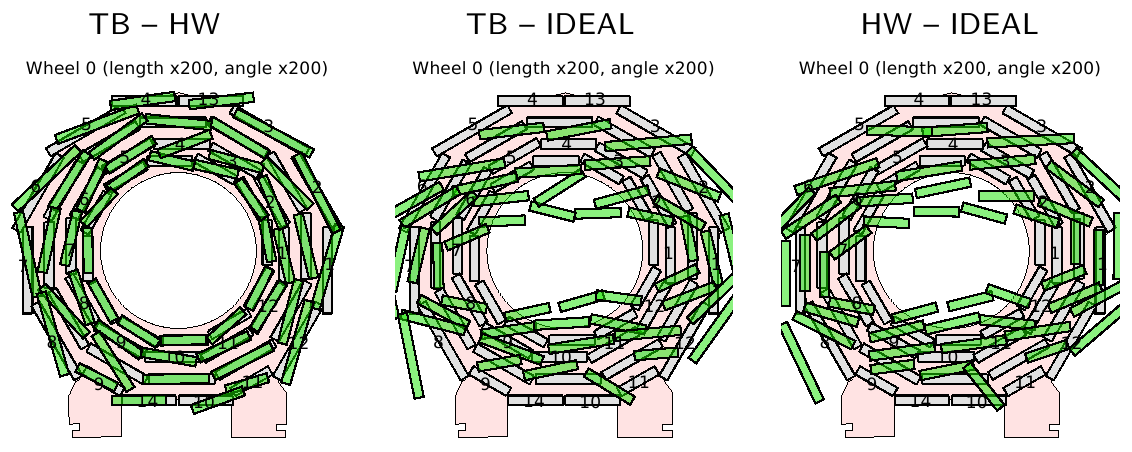
\includegraphics[width=\linewidth]{tb-hw_wheel0.png}

\vfill
\item But the remaining differences are significant: see next page
\end{itemize}
\end{frame}

\begin{frame}
\frametitle{Example: muon barrel twist}
\begin{columns}
\column{0.45\linewidth}
Histograms of $r\phi$ (local $x$) TB-minus-HW differences, separated by wheel

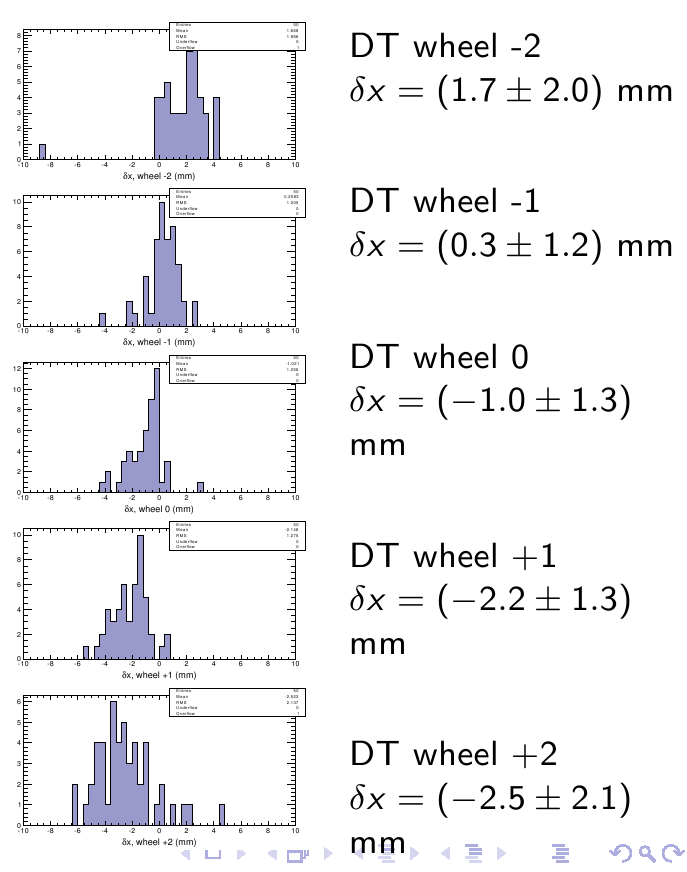
\includegraphics[width=\linewidth]{twist1.png}

\column{0.65\linewidth}
\begin{itemize}\setlength{\itemsep}{0.1 cm}
\item 5-chamber groups from wheel $-$2 \\ to wheel $+$2 seem to be coherently rotated: about 4~mm end-to-end
\item barrel also compressed in $z$ by about 4~mm end-to-end (less relevant for physics)
\item $\mathcal{O}(1.3\mbox{ mm})$ individual-chamber variations
\item<2> Same trends in all four stations (if from the
  tracker, it would grow with radius)
\end{itemize}

\vfill

\only<1>{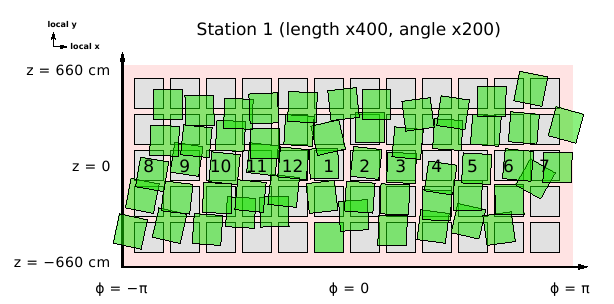
\includegraphics[width=\linewidth]{twist3_station1.png}}
\only<2>{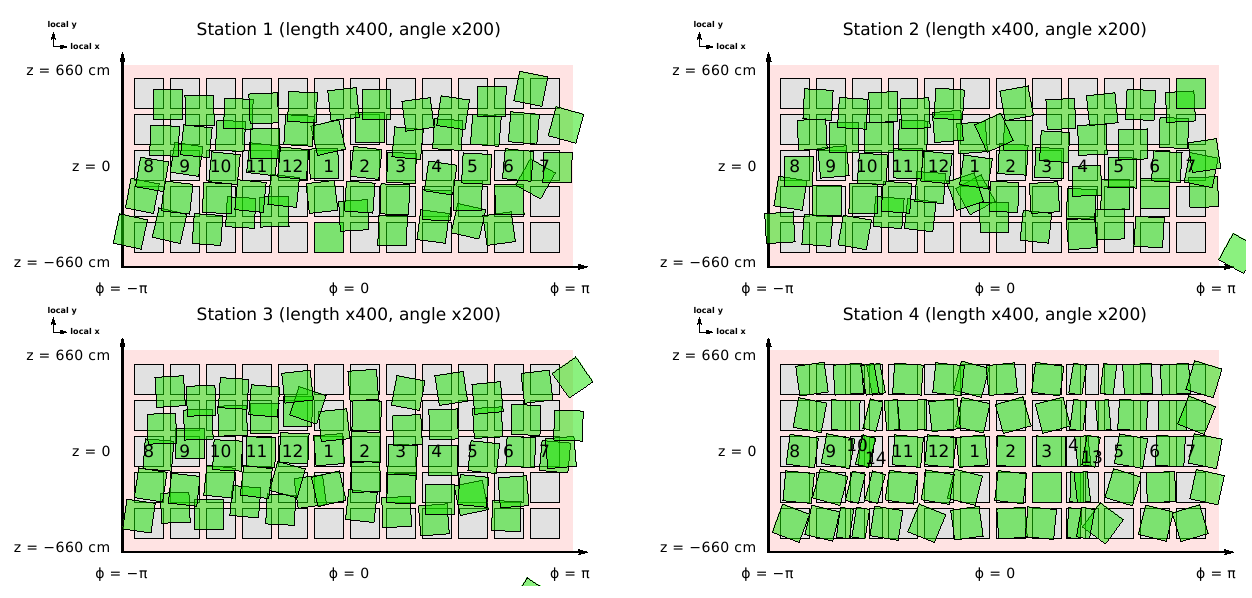
\includegraphics[width=\linewidth]{twist3.png}}
\end{columns}
\end{frame}

\begin{frame}
\frametitle{Example: muon barrel twist}
\begin{itemize}
\item On the next few pages, I'll show the effect of this possible
  systematic misalignment on $Z'$
\item Express its effect on curvature $\kappa = q/p_T$, which is both
  meaningful for physics and easy to relate to alignment errors:
\[ \Delta \kappa \propto \Delta (r\phi) \mbox{ at a specified radius} \]

In barrel station 1 (4.2~m from beamline), $\displaystyle \Delta \kappa \approx 0.1 \frac{c/\mbox{TeV}}{\mbox{mm}} \, \Delta (r\phi)$

\item Studied the effect by twisting the IDEAL barrel geometry (no misalignment in endcap)

\begin{center}
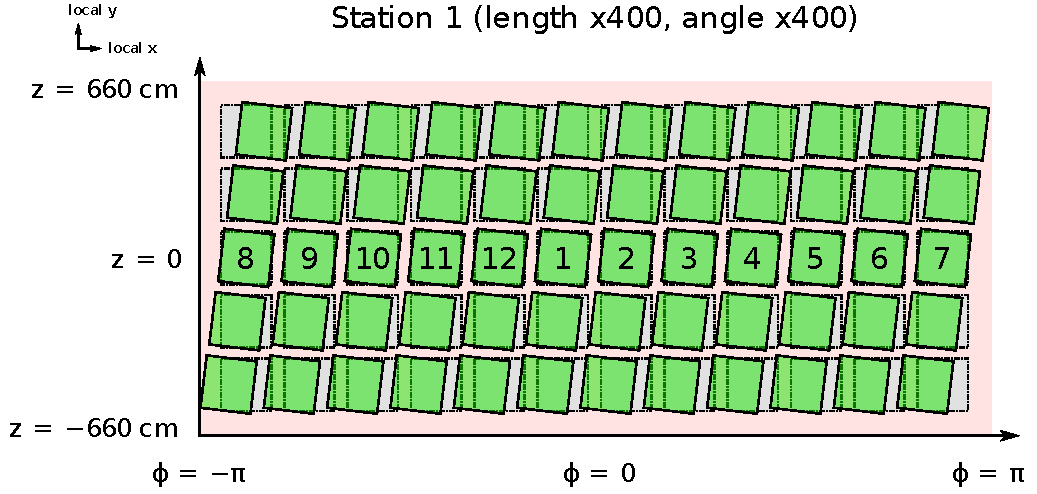
\includegraphics[width=0.5\linewidth]{twist_station1.pdf}
\end{center}
\end{itemize}
\end{frame}

\begin{frame}
\frametitle{Example: muon barrel twist}

\vspace{-0.2 cm}
\begin{columns}
\column{0.5\linewidth}
\begin{center}
Ideal
\end{center}
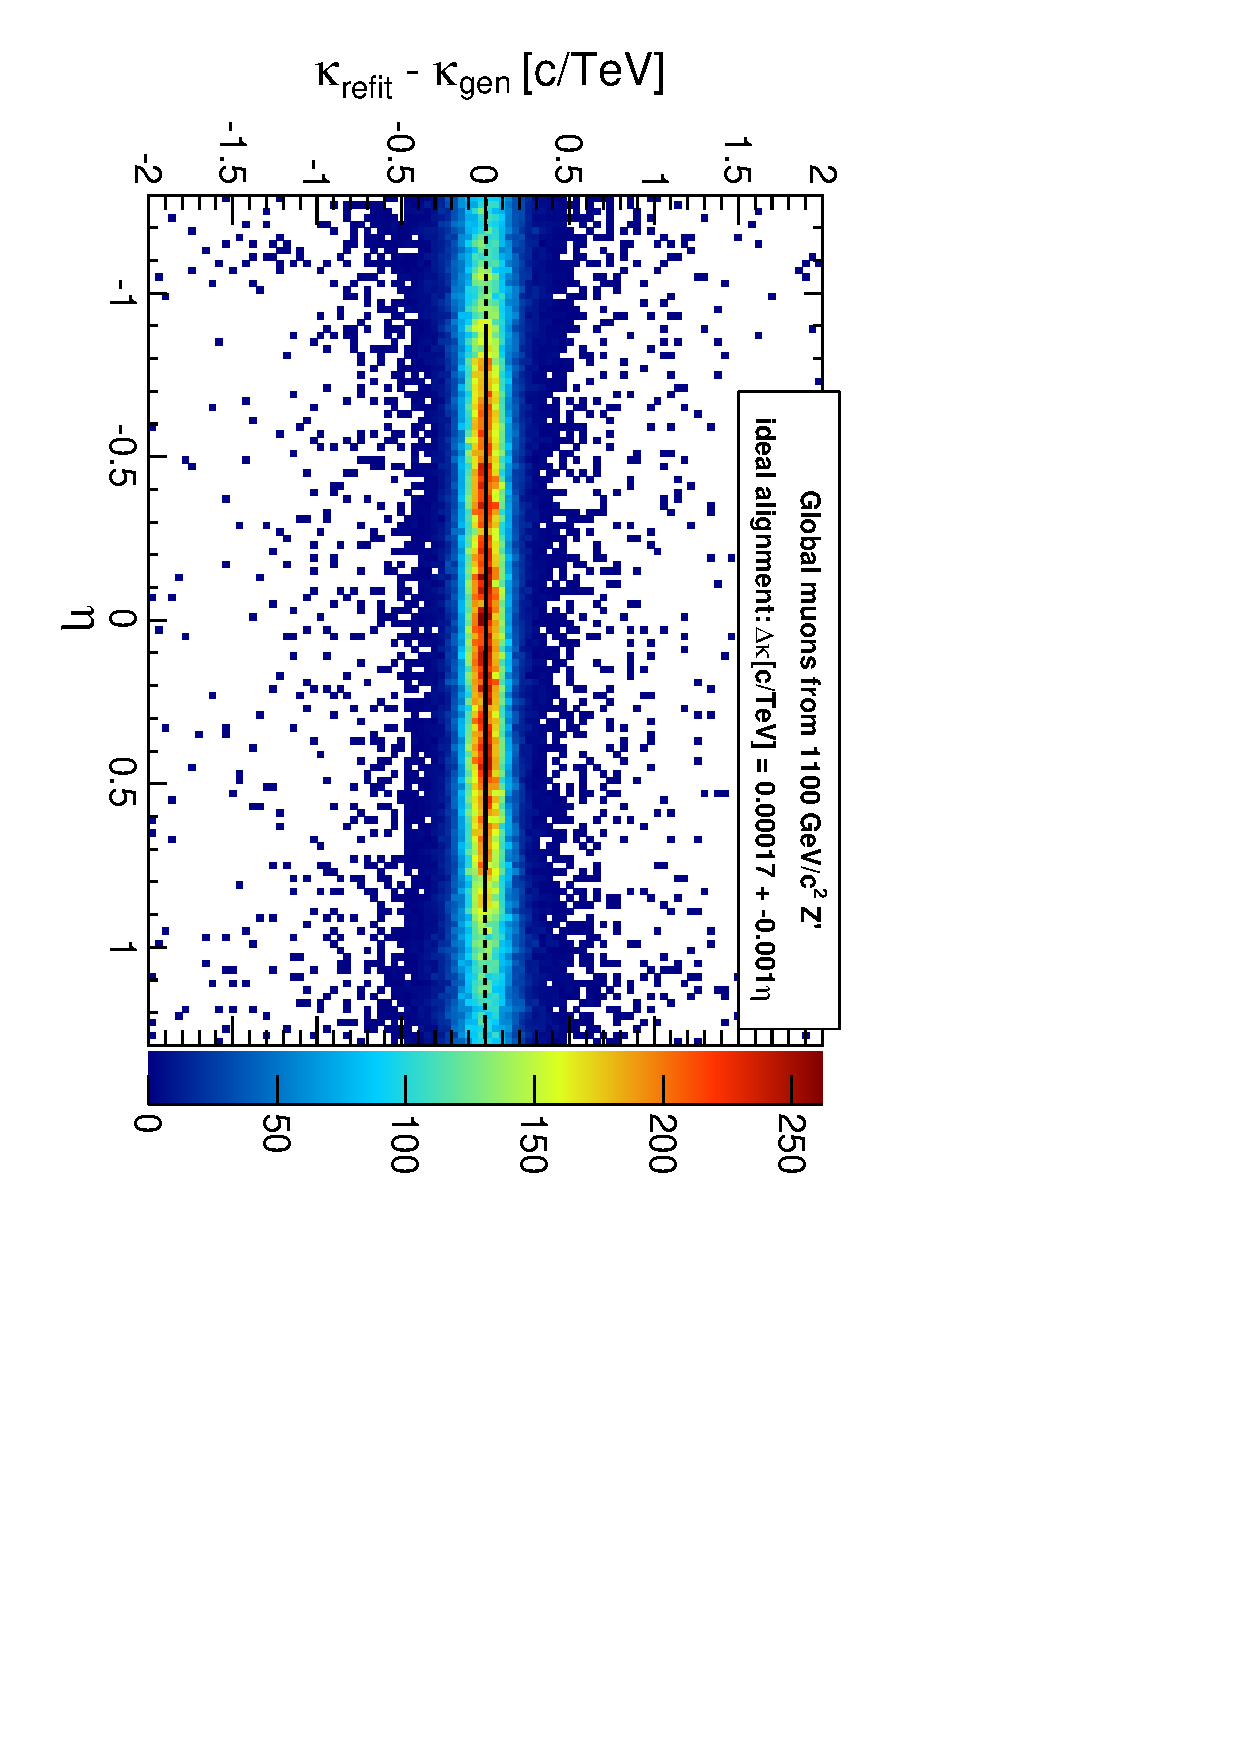
\includegraphics[height=\linewidth, angle=90]{curvbias_vseta_ideal_1100_GlobalMuons2.pdf}

\column{0.5\linewidth}
\begin{center}
0.5~mrad twist
\end{center}
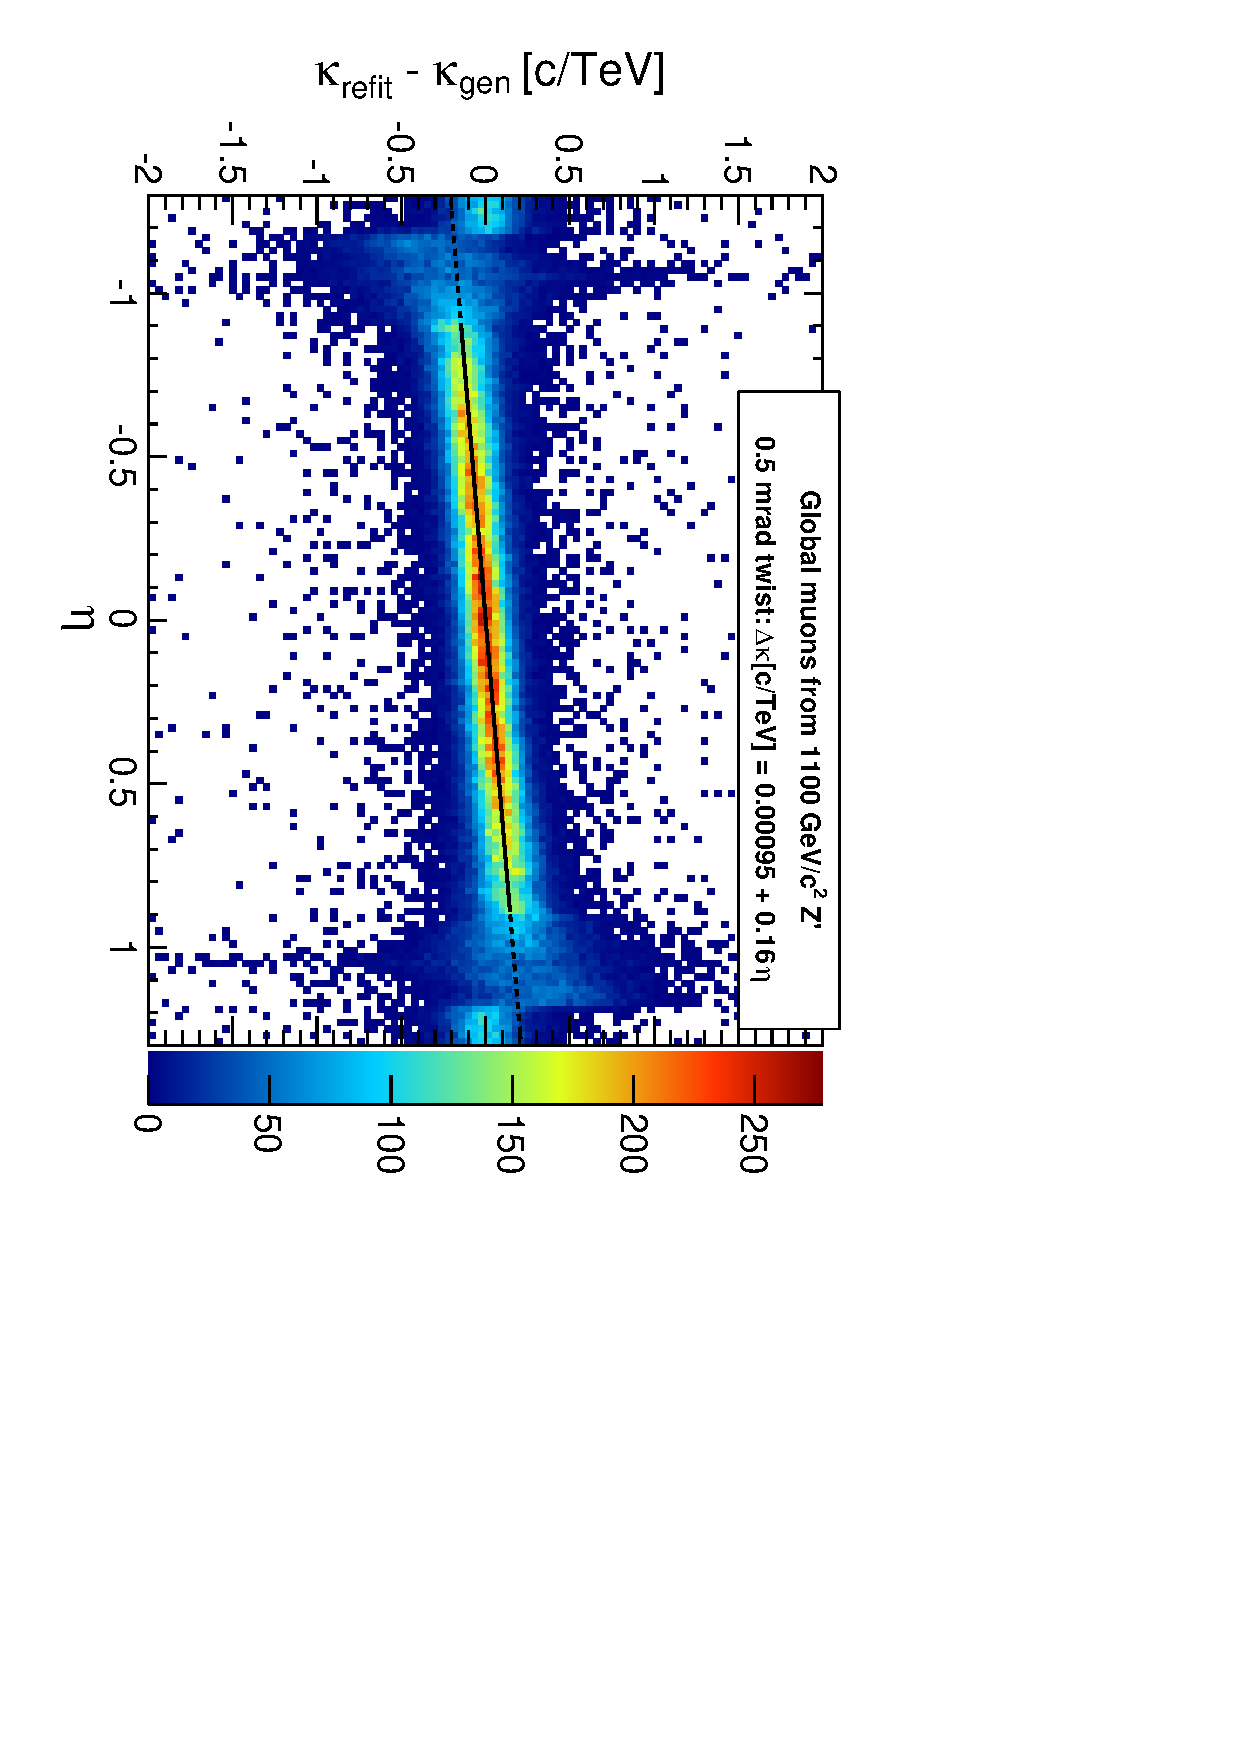
\includegraphics[height=\linewidth, angle=90]{curvbias_vseta_twist0_5mrad_1100_GlobalMuons2.pdf}
\end{columns}

\vspace{-0.25 cm}
\begin{columns}
\column{0.33\linewidth}
\begin{center}
GlobalMuons

\vspace{-0.2 cm}
\end{center}
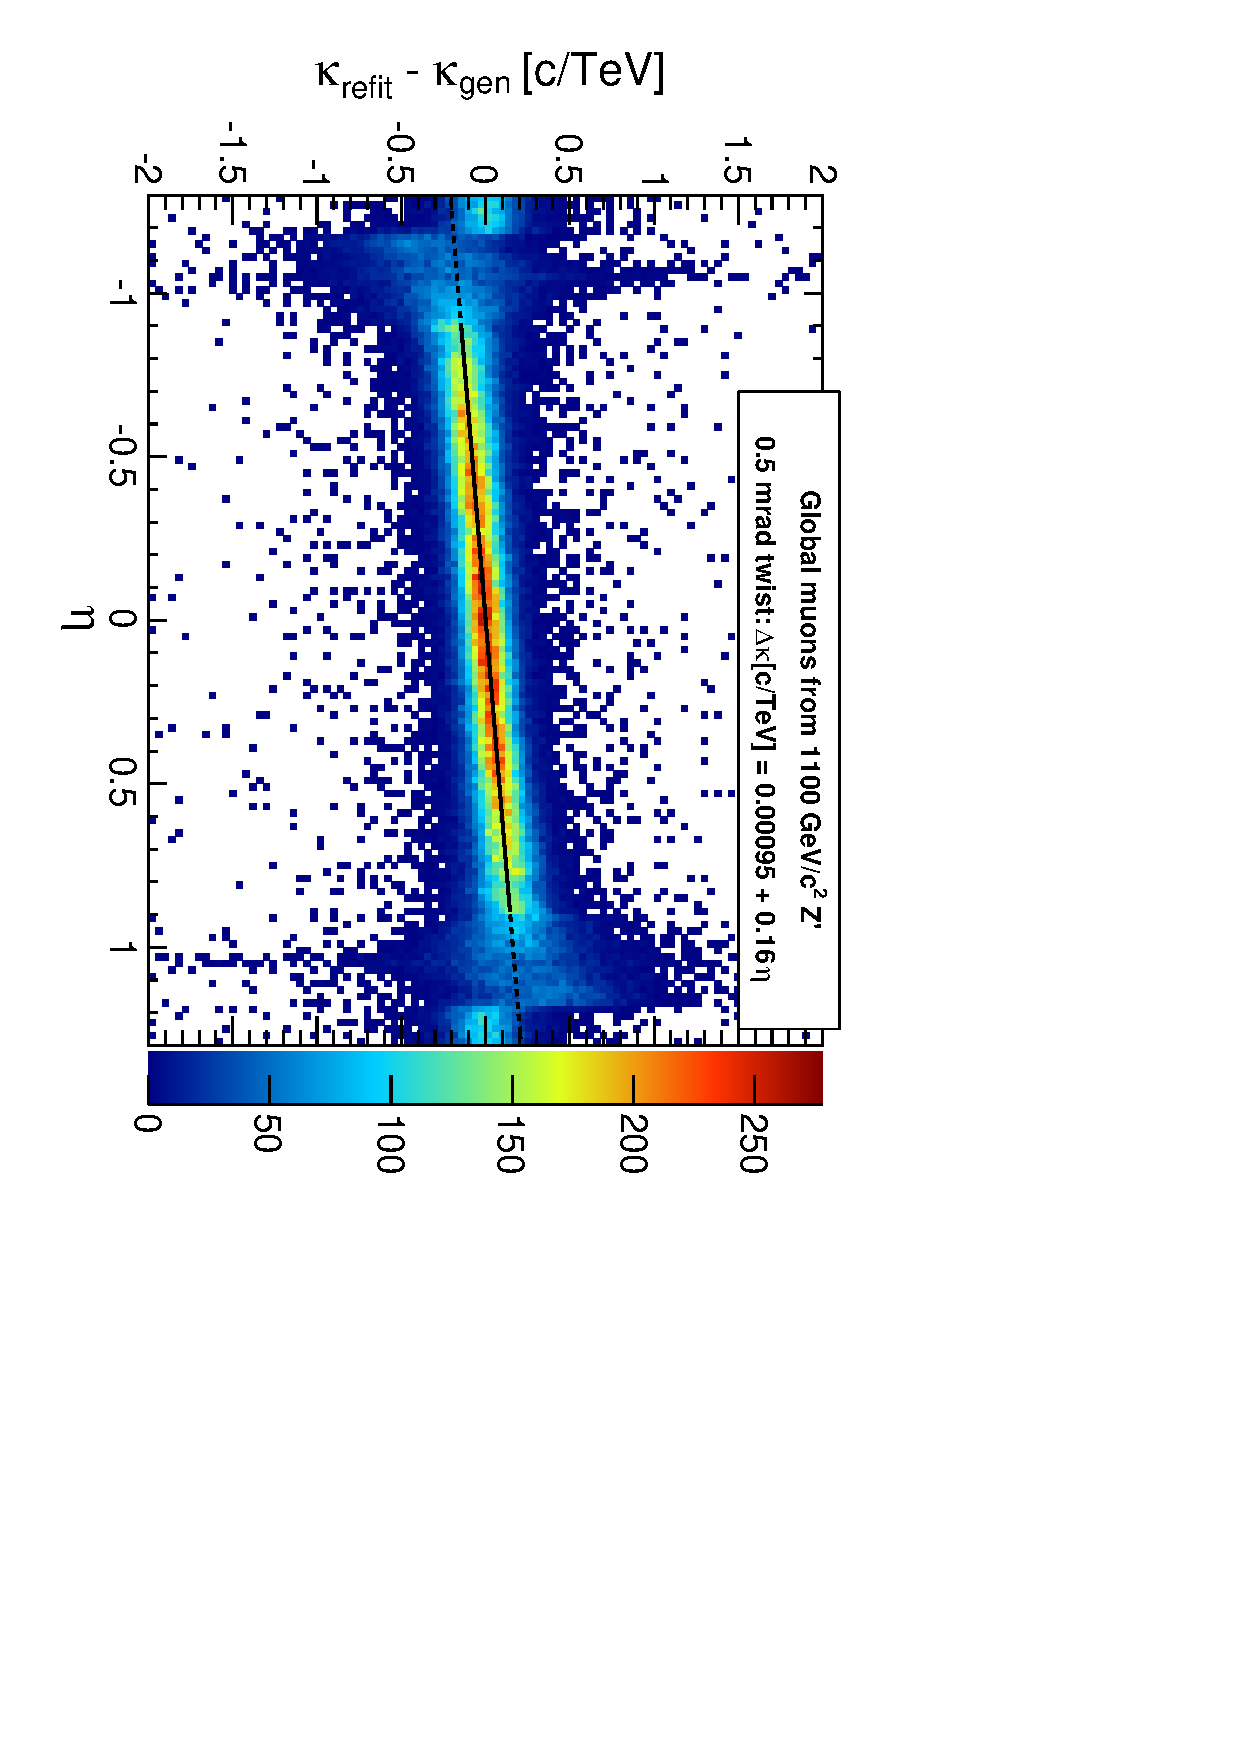
\includegraphics[height=\linewidth, angle=90]{curvbias_vseta_twist0_5mrad_1100_GlobalMuons2.pdf}

\column{0.33\linewidth}
\begin{center}
Picky

\vspace{-0.2 cm}
\end{center}
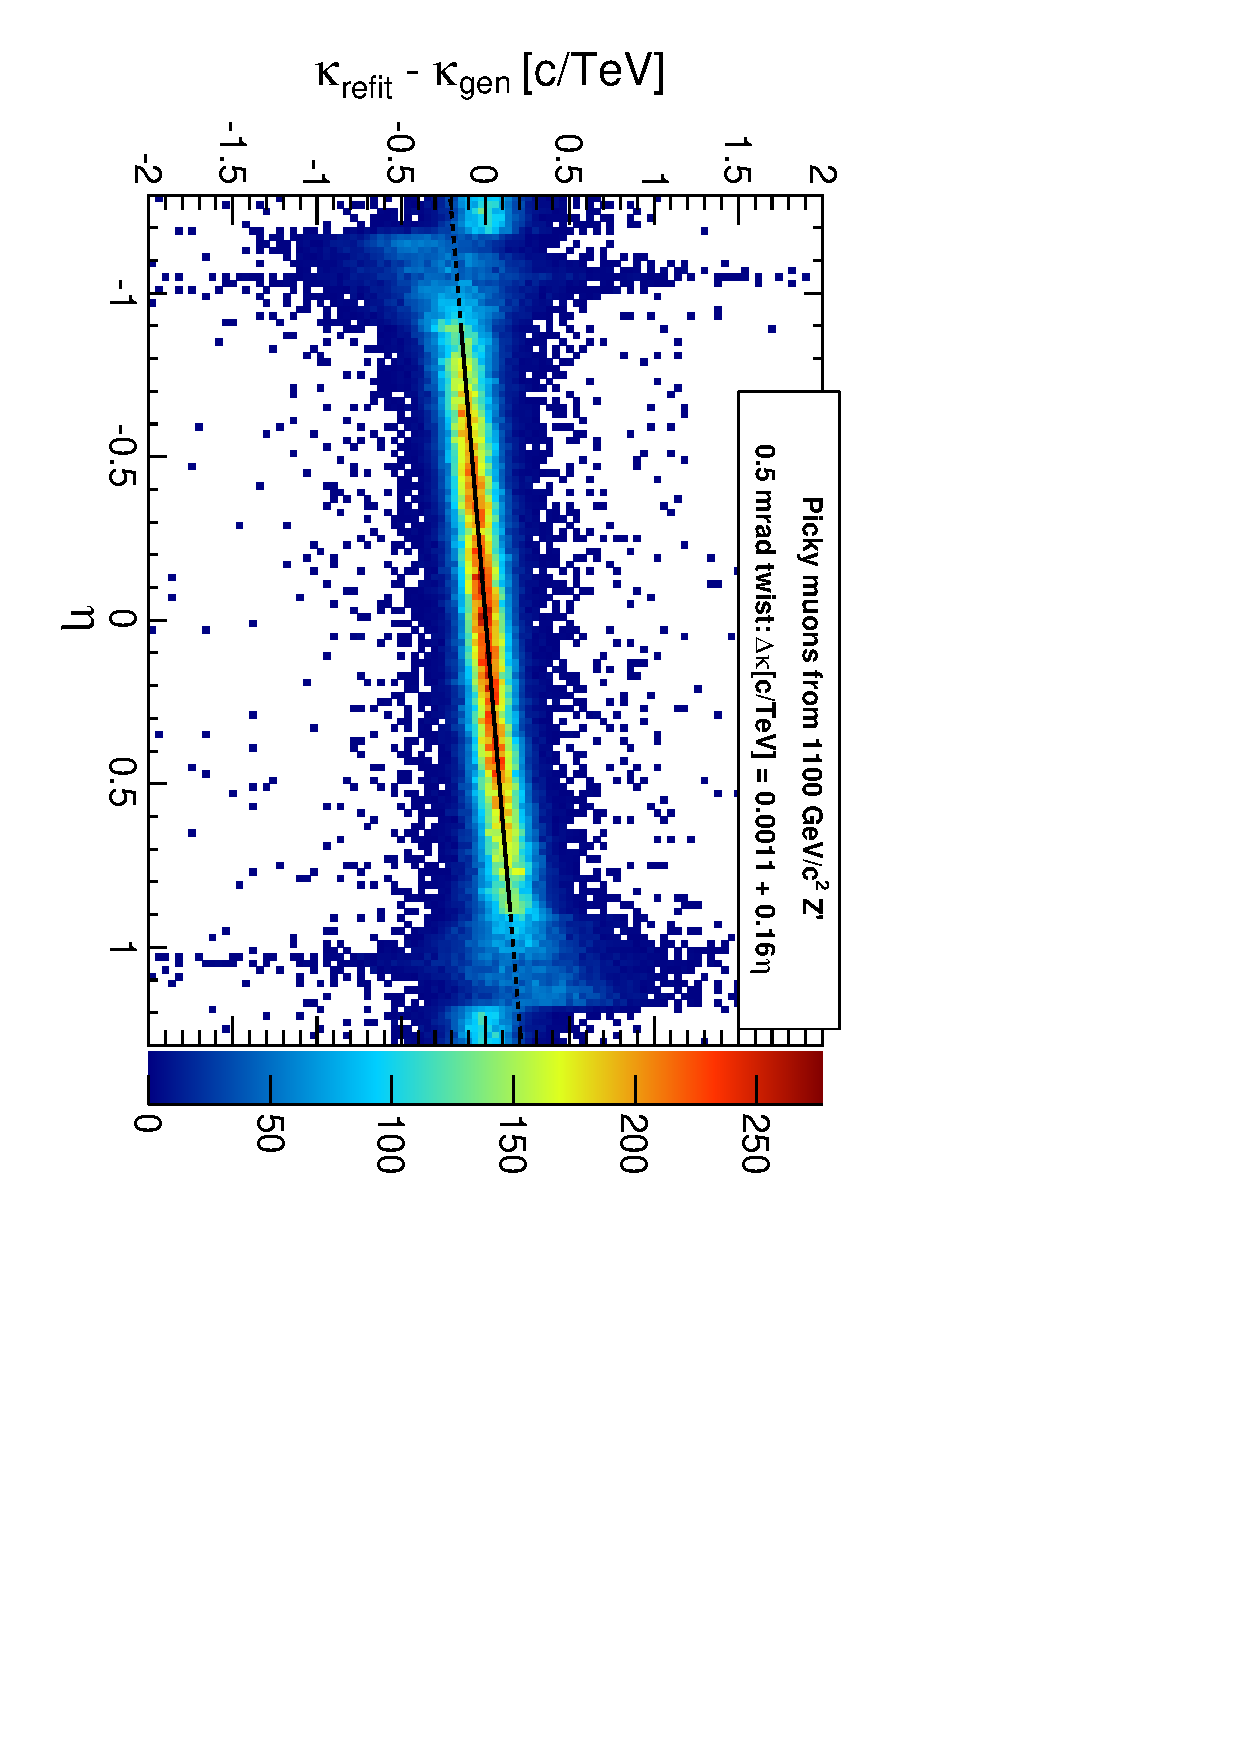
\includegraphics[height=\linewidth, angle=90]{curvbias_vseta_twist0_5mrad_1100_TeVMuons2picky.pdf}

\column{0.33\linewidth}
\begin{center}
FirstStation

\vspace{-0.2 cm}
\end{center}
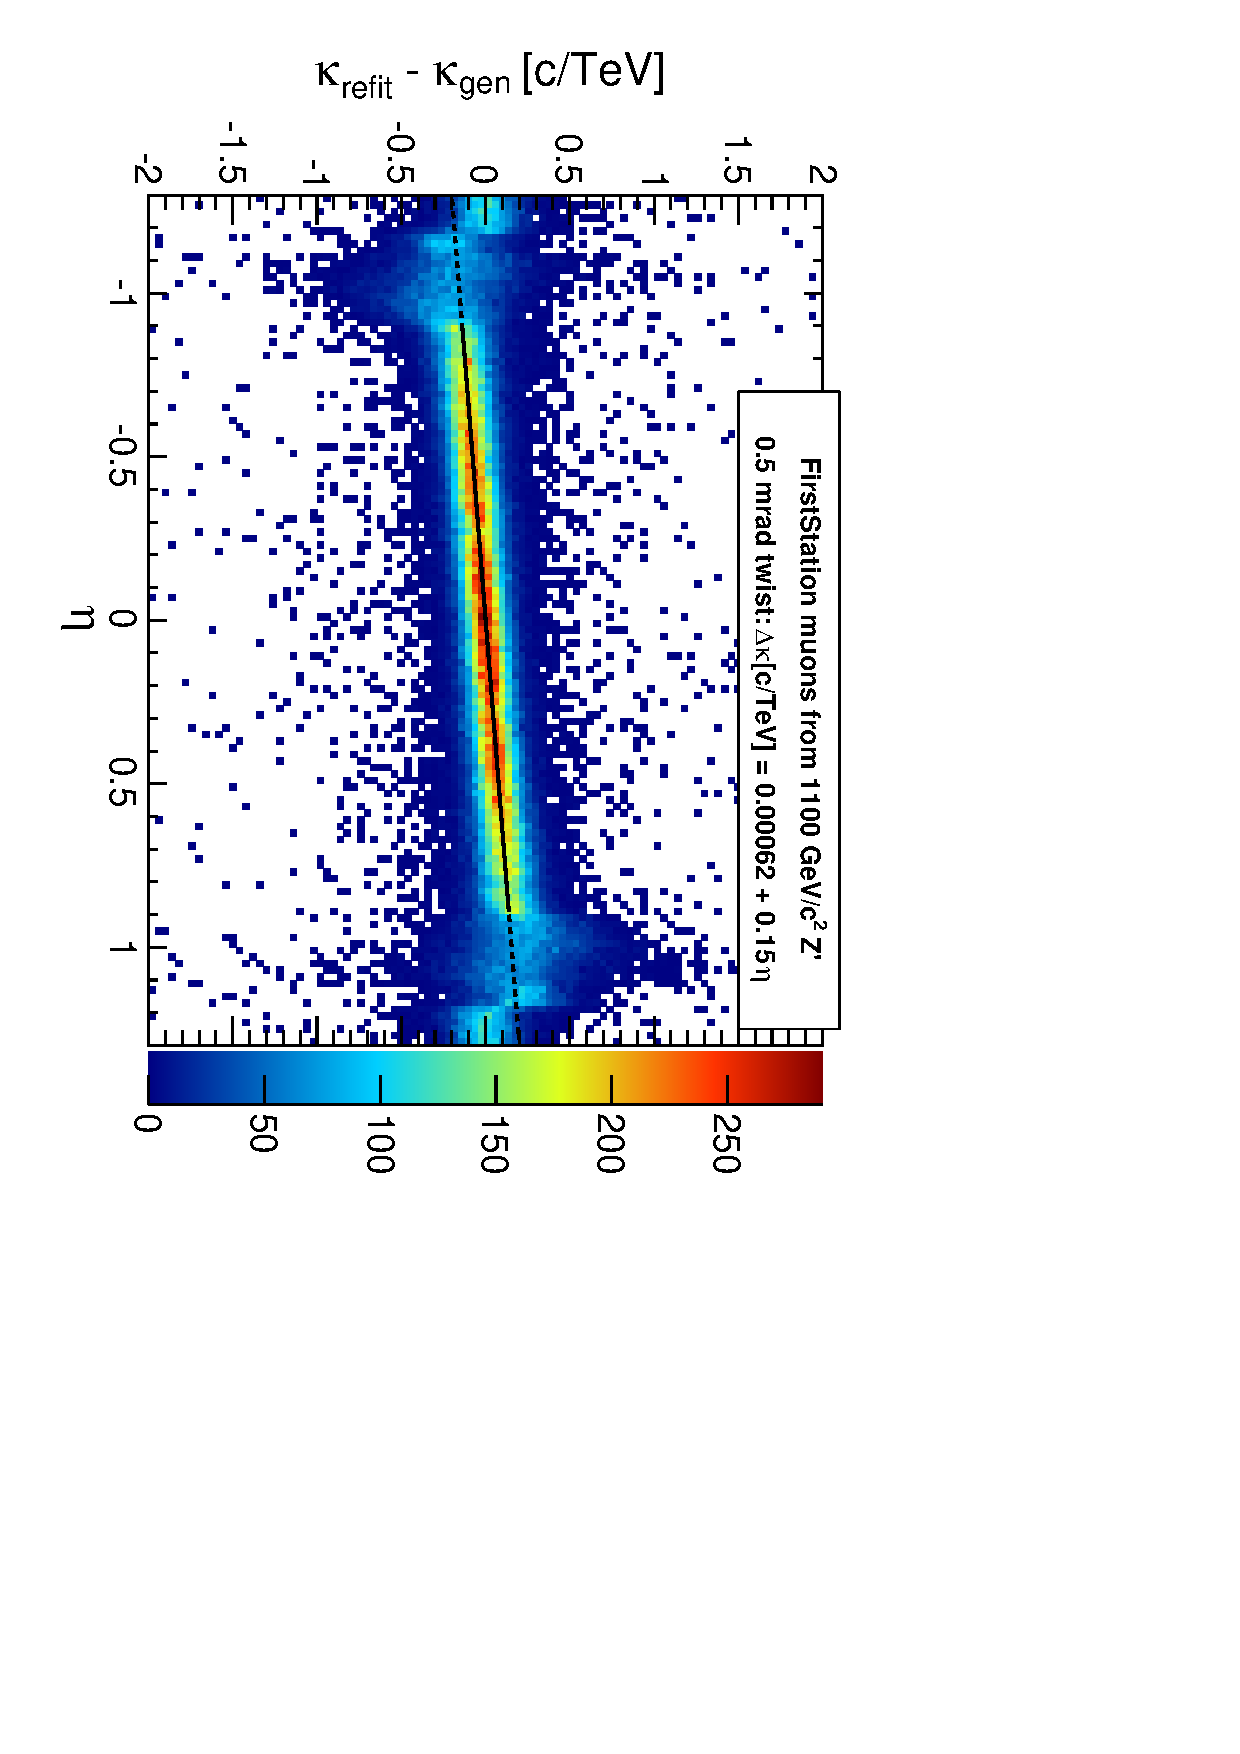
\includegraphics[height=\linewidth, angle=90]{curvbias_vseta_twist0_5mrad_1100_TeVMuons2firstHit.pdf}
\end{columns}
\end{frame}

\begin{frame}
\frametitle{Example: muon barrel twist}
\begin{itemize}
\item In this plot, color scale is average $\Delta\kappa$ in $c$/TeV (we get to see the bias, but not the width of the distribution)
\item Lines are contours of the 2-D fit result (bilinear ansatz)
\end{itemize}
\begin{center}
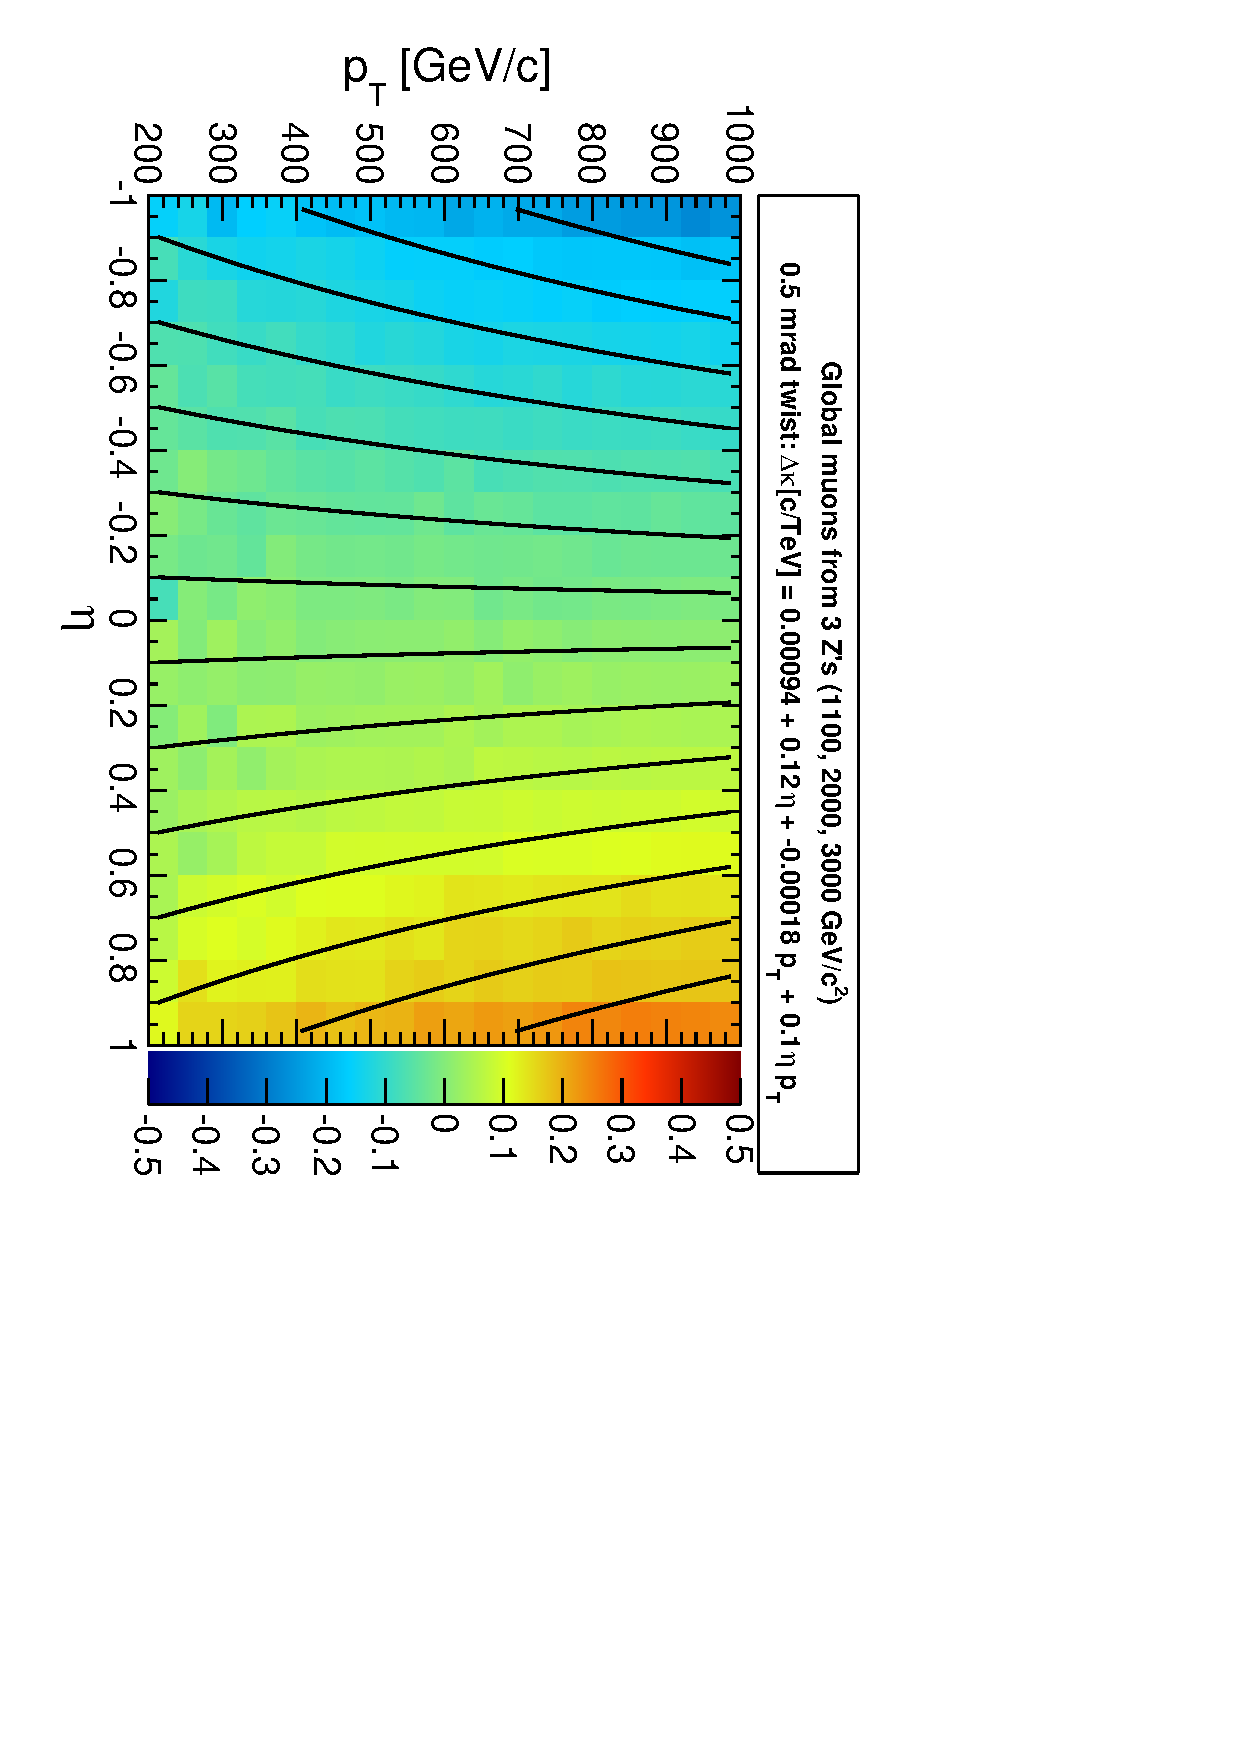
\includegraphics[height=0.9\linewidth, angle=90]{trackdistort2d_twist0_5mrad_GlobalMuons2.pdf}
\end{center}
\end{frame}

\begin{frame}
\frametitle{Example: muon barrel twist}
\begin{itemize}
\item Effect on $Z'$ mass (quantity of interest is $(m_\s{refit} - m_\s{gen})/m_\s{gen}$)
\item Key variables: $(\eta_\s{lead} - \eta_\s{sublead})$ and $q_\s{lead}$

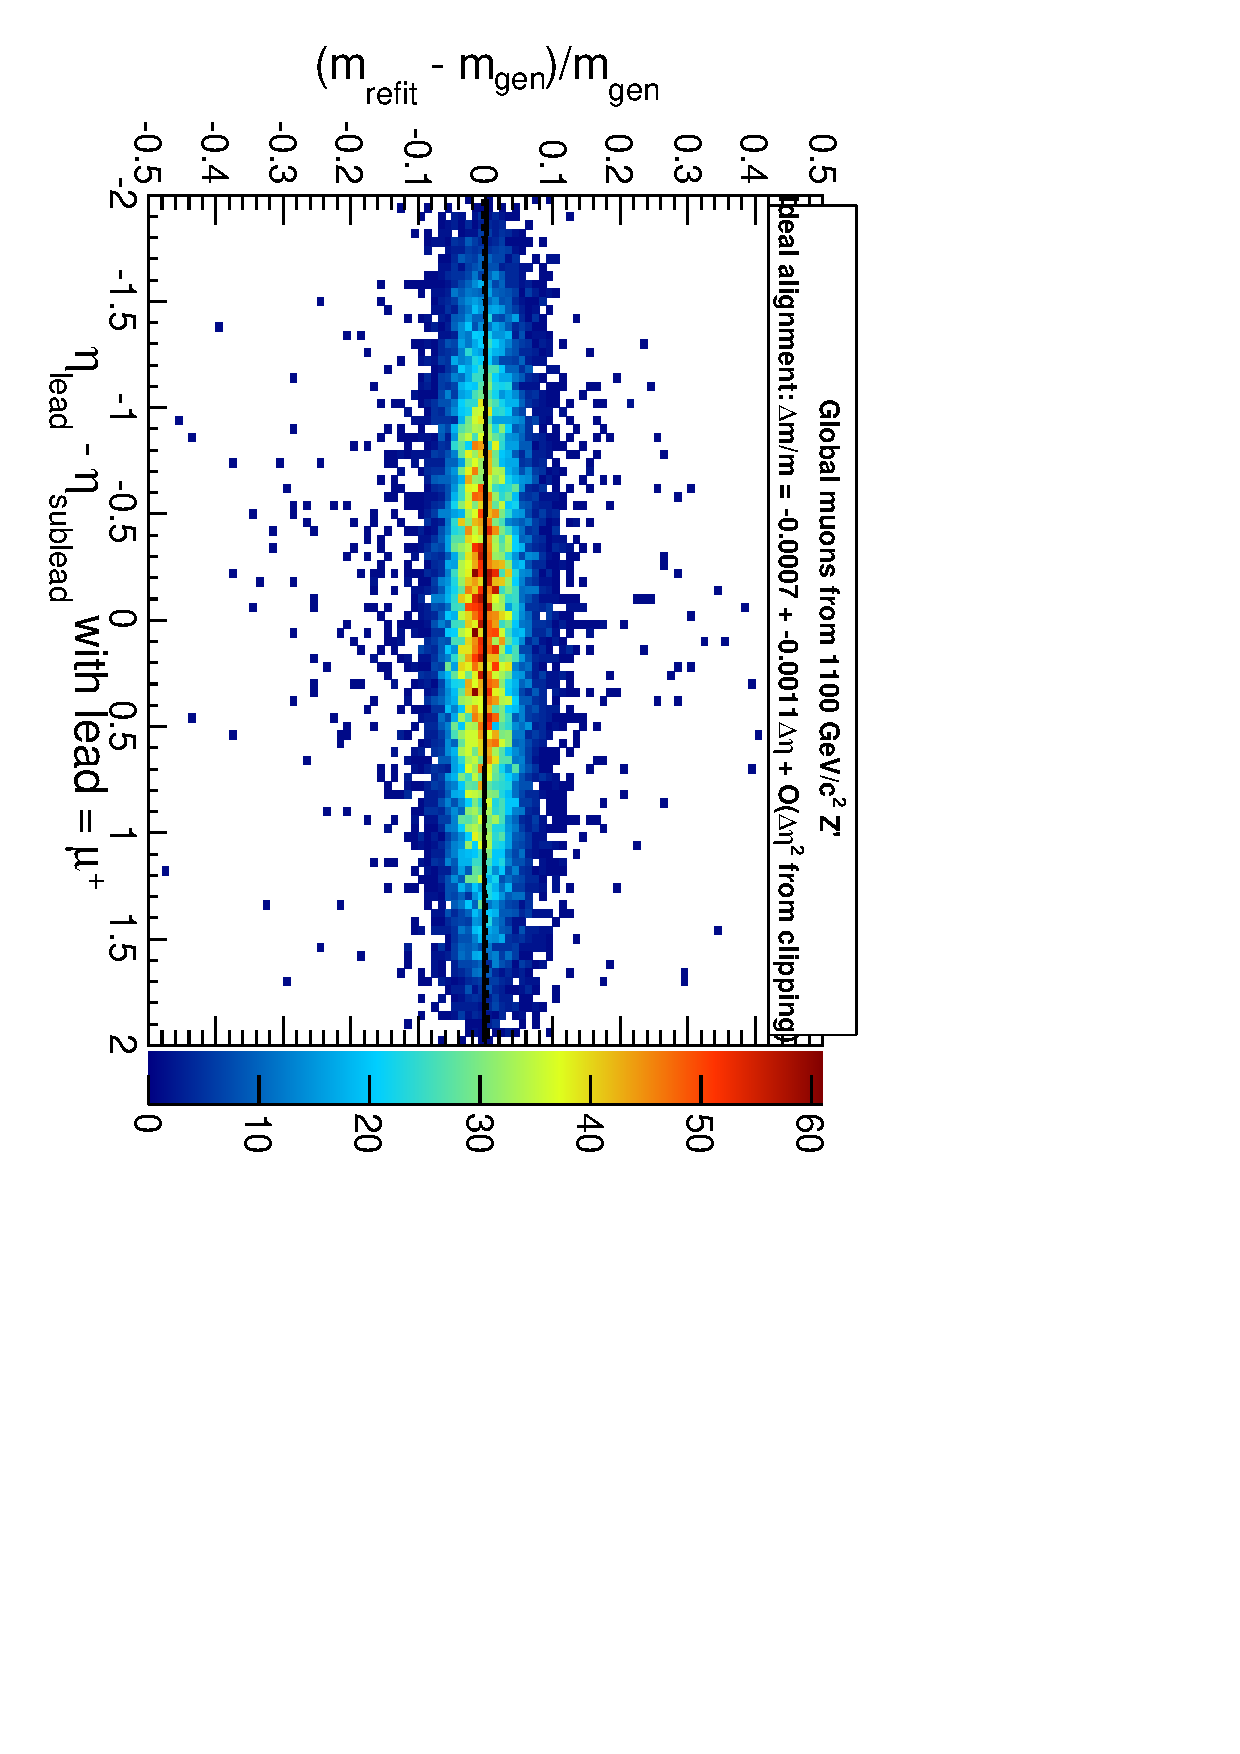
\includegraphics[height=0.49\linewidth, angle=90]{massbias_ideal_1100_GlobalMuons2_plus.pdf}
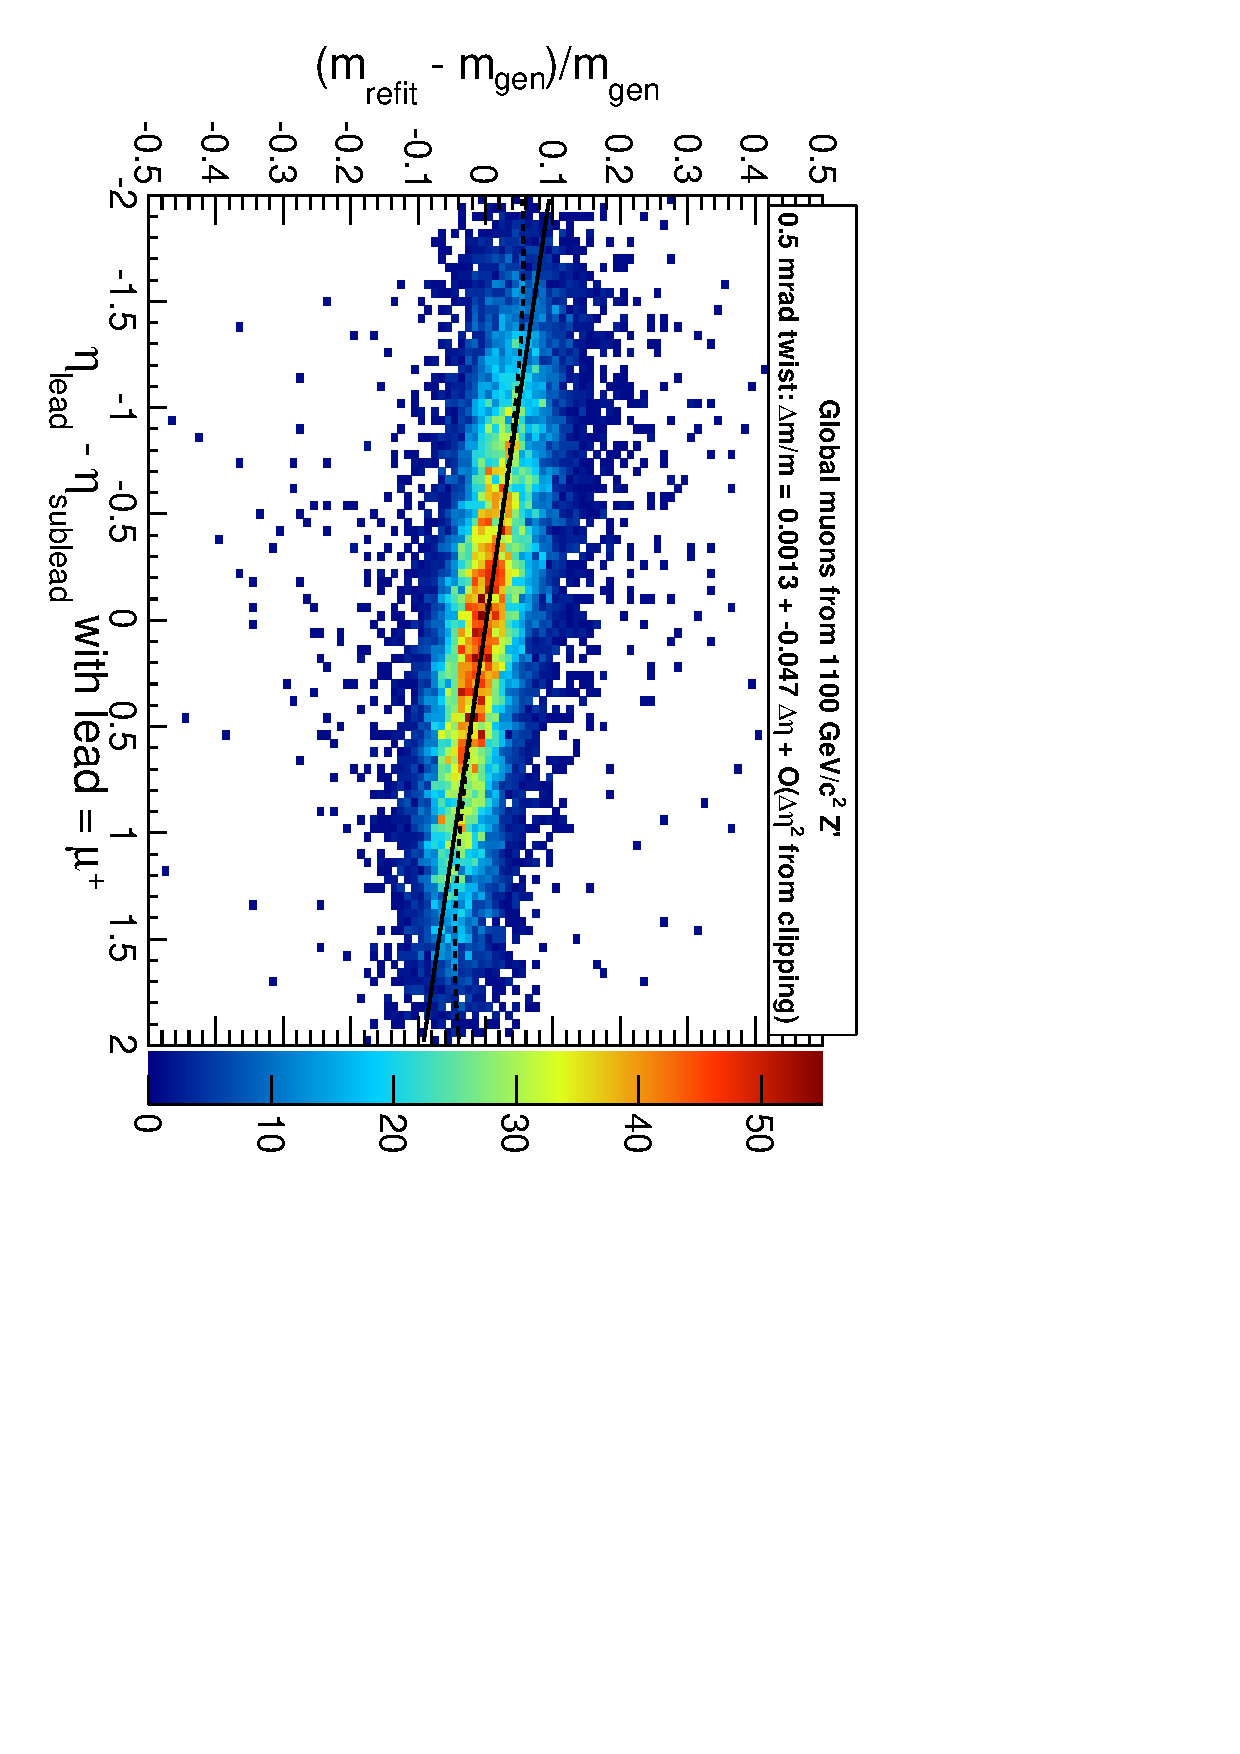
\includegraphics[height=0.49\linewidth, angle=90]{massbias_twist0_5mrad_1100_GlobalMuons2_plus.pdf}

\item 1-D distributions for $Z'$ with $|\eta| < 1$, $m_{Z'}$ = 1.1, 2, 3~TeV/$c^2$

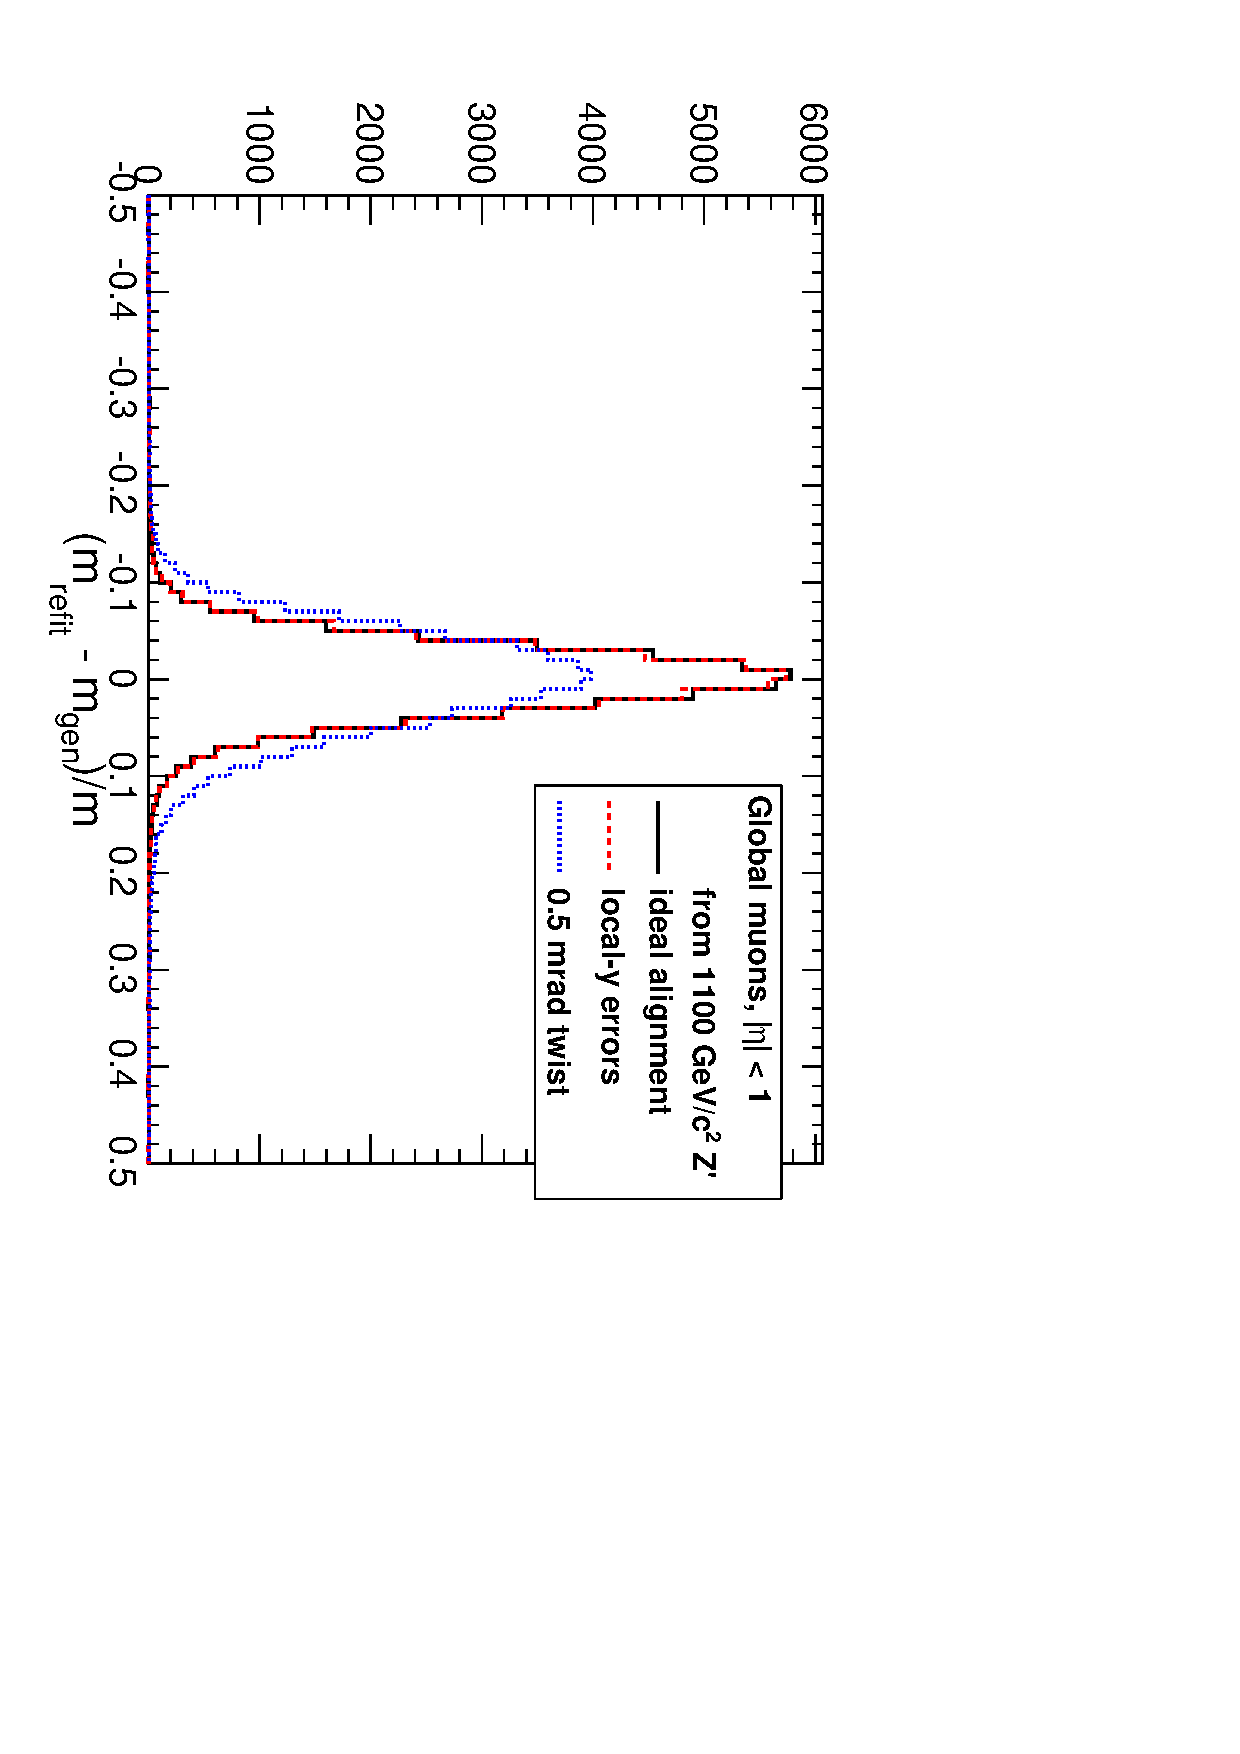
\includegraphics[height=0.32\linewidth, angle=90]{massdistribution_1100_GlobalMuons2.pdf}
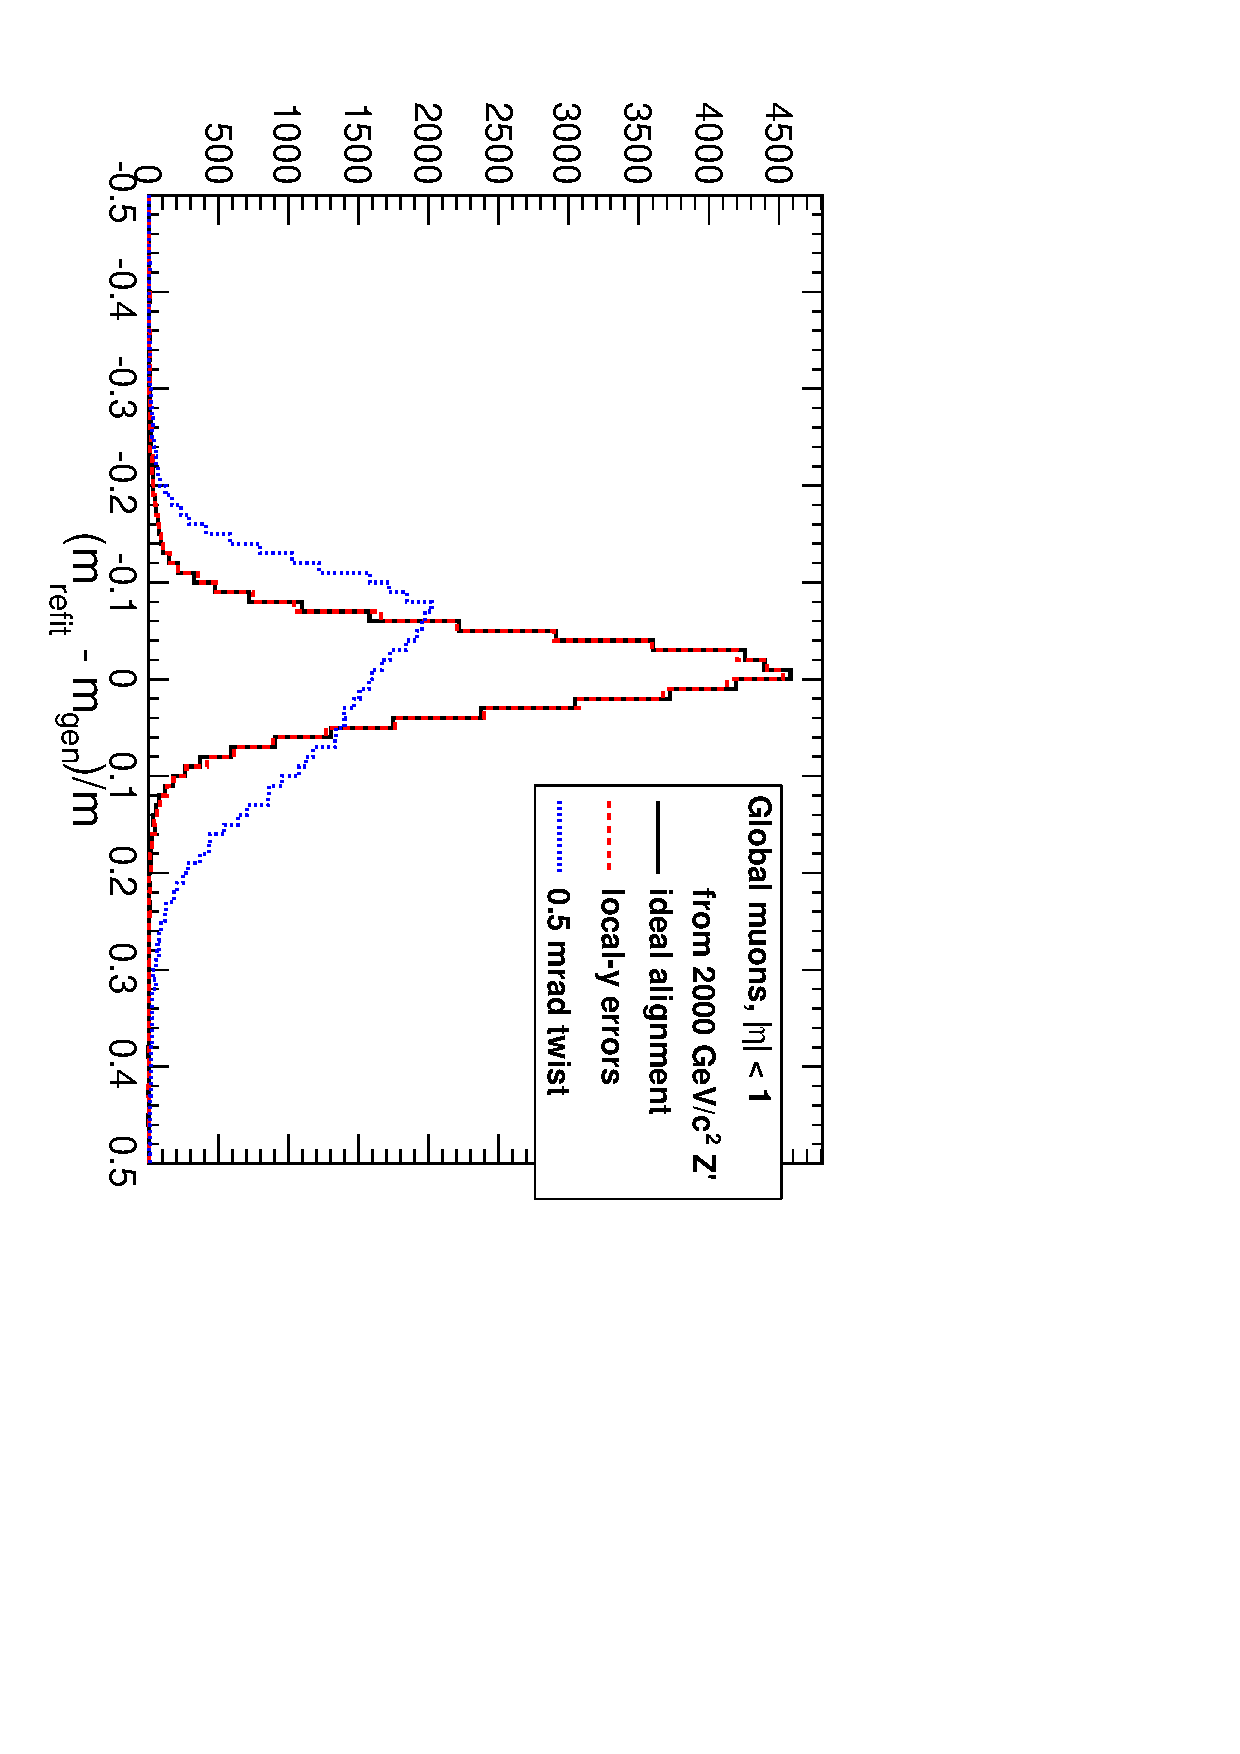
\includegraphics[height=0.32\linewidth, angle=90]{massdistribution_2000_GlobalMuons2.pdf}
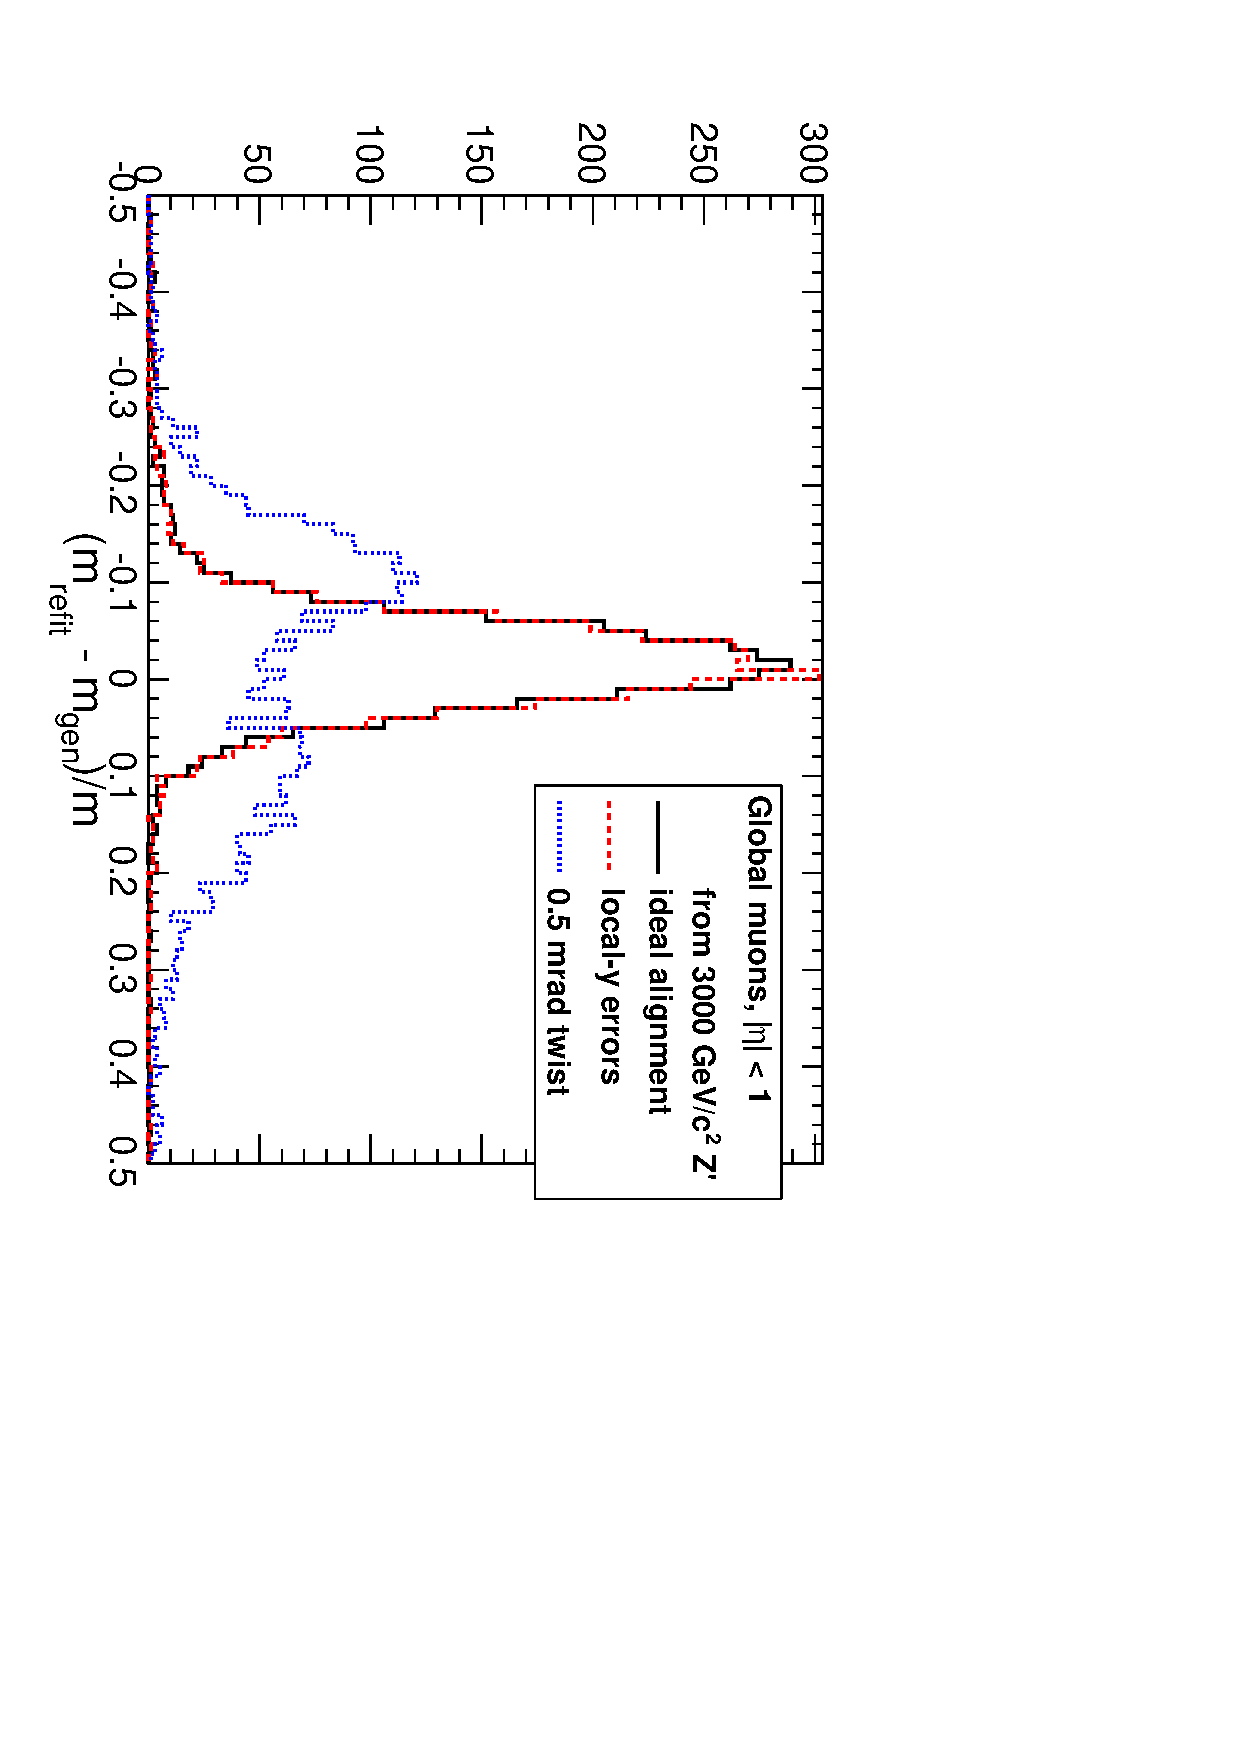
\includegraphics[height=0.32\linewidth, angle=90]{massdistribution_3000_GlobalMuons2.pdf}
\end{itemize}
\end{frame}

\begin{frame}
\frametitle{How to proceed}
\begin{itemize}
\item Naturally, the tracker and muon alignment groups will continue
  their studies to improve resolutions and reduce uncertainties about biases
\end{itemize}

\vspace{0.2 cm}
\hspace{-0.83 cm} \textcolor{darkblue}{\large Physics-level tests}

\begin{itemize}
\item \textcolor{darkblue}{Split cosmics:} compare $\kappa$ of top and
  bottom halves of a reconstructed cosmic ray
\begin{itemize}
\item CRAFT-08 with $p_T > 200$~GeV/$c$ was sensitive to 0.6~$c$/TeV
\item relaxing impact parameter cuts and larger cosmics samples could
  increase reach to 0.1~$c$/TeV or better\ldots
\item twist would show up as $\Delta \kappa = (0.13\mbox{ $c$/TeV}) \cot\theta$
\end{itemize}

\item \textcolor{darkblue}{Cosmics endpoint:} distribution of cosmic
  rays $\to$ 0 as $\kappa \to 0$, so offset of the minimum of the
  distribution in $\kappa$ indicates a bias
\begin{itemize}
\item CRAFT-08 sensitive to 0.05~$c$/TeV
\item can it be binned in $\cot\theta$?
\end{itemize}

\item \textcolor{darkblue}{$Z$ mass constraint:} most collisions
  tracks with $p_T > 200$~GeV/$c$ come from boosted $Z$; starts to be sensitive at about \mbox{1~fb$^{-1}$ (backups)\hspace{-1 cm}}
\end{itemize}
\end{frame}

\begin{frame}
\frametitle{$Z'$ analysis specifically}
\begin{itemize}
\item First, a question: will a detector resolution (or bounds on
  detector resolutions) be assumed in the peak-search fit?
\begin{itemize}
\item if yes, then we need to minimize {\it uncertainty} in resolution
\item in either case, resolution must be made as narrow as possible
\end{itemize}

\item Suppose that we still have a several-fold ambiguity, such as TB
  versus HW in the barrel (two distinct possibilities)
\begin{itemize}
\item we could model the difference in MC with specialized scenarios,
  like I showed here, to understand the consequences of choosing the
  wrong one

\vspace{0.2 cm}
this could be a systematic uncertainty

\vspace{0.2 cm}
\item we could search for peaks with both real-data geometries, though
  that would reduce the statistical significance of the result in a
  complicated way
\end{itemize}

\item Opinions?
\end{itemize}
\end{frame}

% AN-2010/059 Calibration of track momentum using dimuon resonances in CMS
% demonstrates 5% precision (in 4 parameters) using 2000 times as many Z events (no hard pT1 cut)

%% \section*{First section}
%% \begin{frame}
%% \begin{center}
%% \Huge \textcolor{blue}{First section}
%% \end{center}
%% \end{frame}

\begin{frame}
\frametitle{Conclusions}
\begin{itemize}
\item Most important issues in alignment to be aware of:
\begin{itemize}\setlength{\itemsep}{0.2 cm}
\item while local misalignments (smearing) are under control, the
  possibility of global distortions (skewing) is still significant

\item MC scenarios cannot encapsulate the latter

\item independent alignments in muon barrel differ by a systematic
  distortion, a twist and a $Z$-compression

\item we can quantify the error introduced by choosing the wrong one,
  but that's a systematic uncertainty, not a resolution

\item to know the resolution, we need to resolve the discrepancies
  between TB and HW alignment methods or measure it with physics-level
  tests
\end{itemize}

\item How this relates to the $Z'$ analysis workflow depends on
  whether the peak-search fit assumes knowledge of detector resolution
  or not
\end{itemize}
\label{numpages}
\end{frame}

\begin{frame}
\frametitle{Backup: resolutions from $Z$}
\begin{itemize}
\item Track momentum scale and resolutions can be determined from
  $Z\to\mu\mu$ (AN-2010/059), but how sensitive is this technique to
  the muons relevant for $Z'$?

\item The good news: most $p_T > 200$~GeV/$c$ muons come from
  $Z$ (below: 1~fb$^{-1}$ Zmumu\_M20\_CTEQ66-powheg GlobalMuons, both in plateau region of HLT\_Mu9; gen-level MC@NLO looks the same)

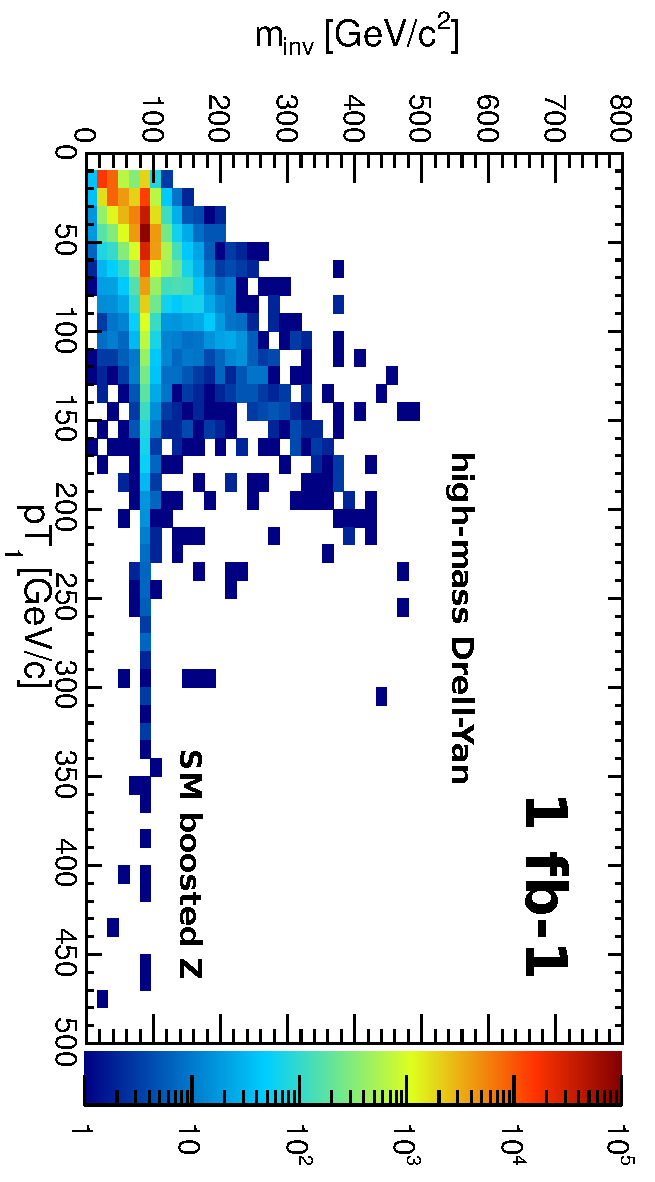
\includegraphics[height=0.9\linewidth, angle=90]{mass_vs_ptone_200.pdf}
\end{itemize}
\end{frame}

\begin{frame}
\frametitle{Backup: resolutions from $Z$}
\begin{columns}
\column{0.7\linewidth}
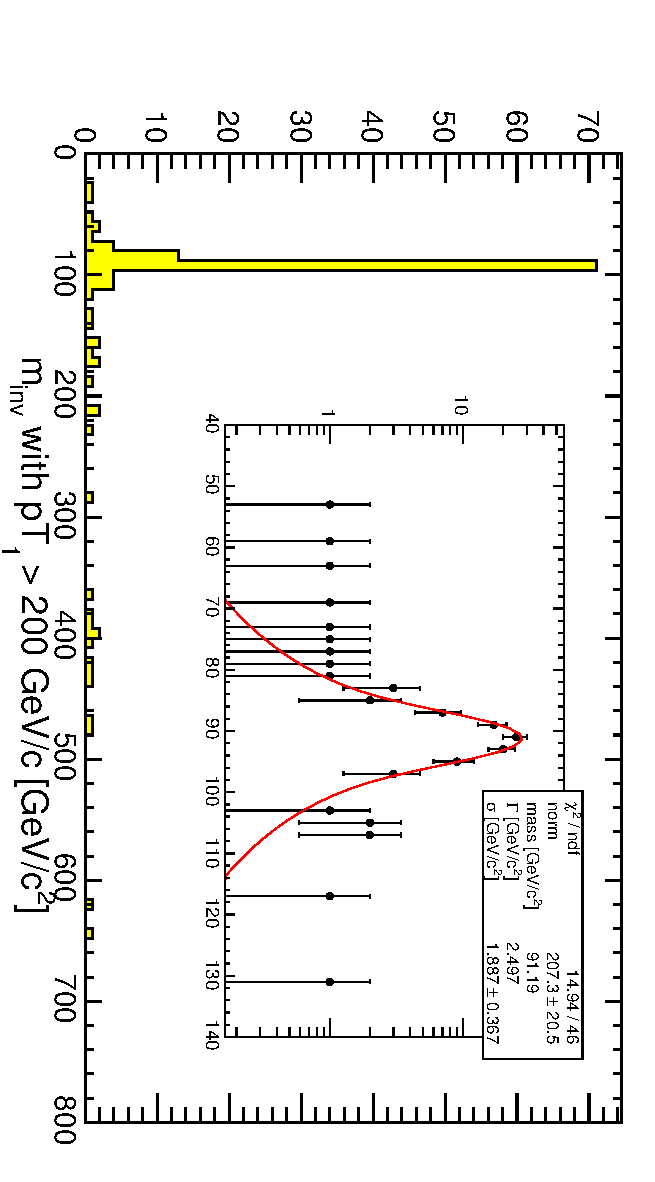
\includegraphics[height=\linewidth, angle=90]{mass_200.pdf}

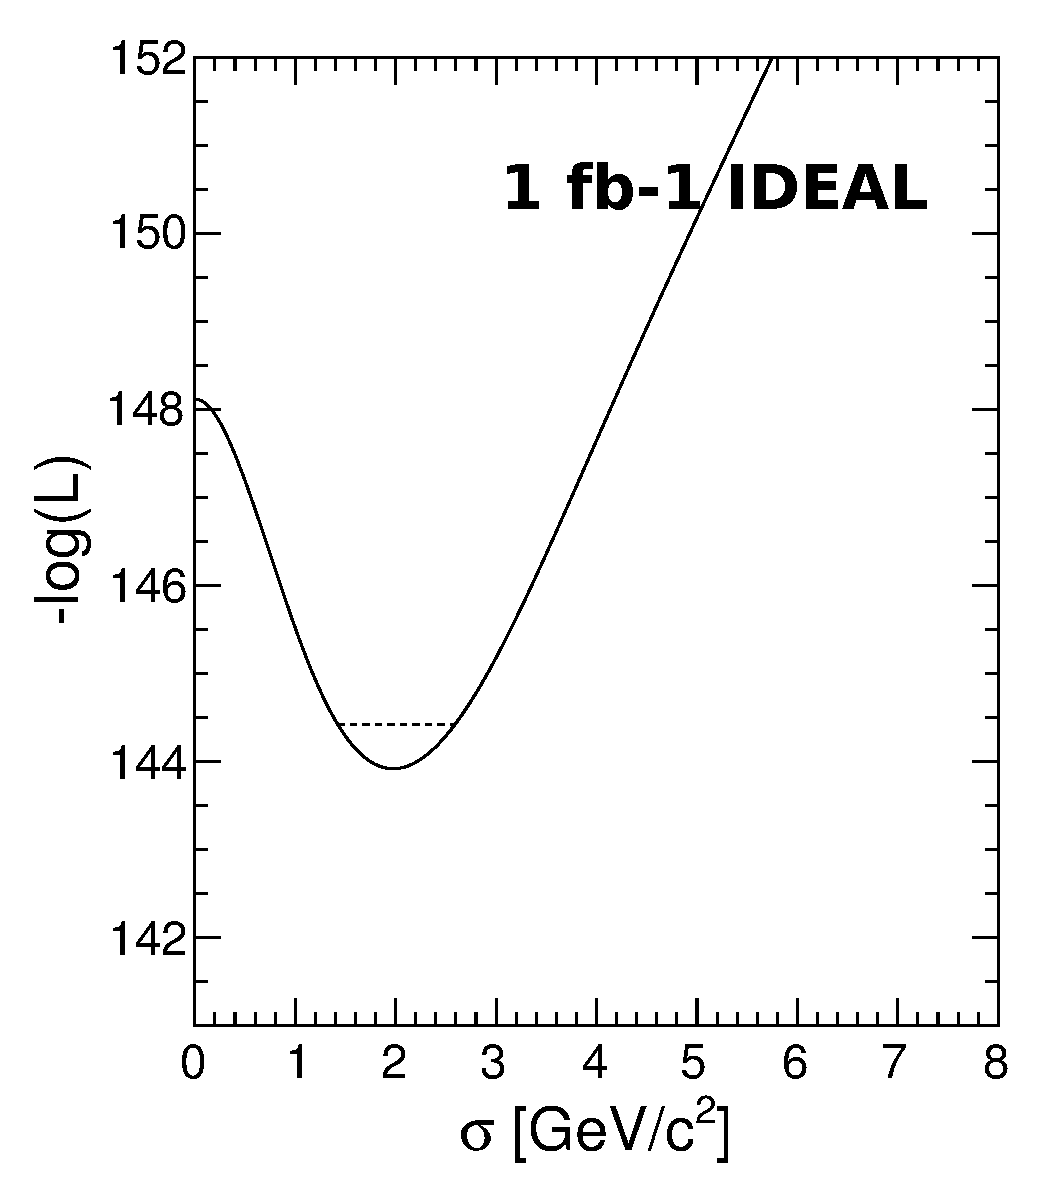
\includegraphics[width=0.49\linewidth]{loglike_ideal.pdf}
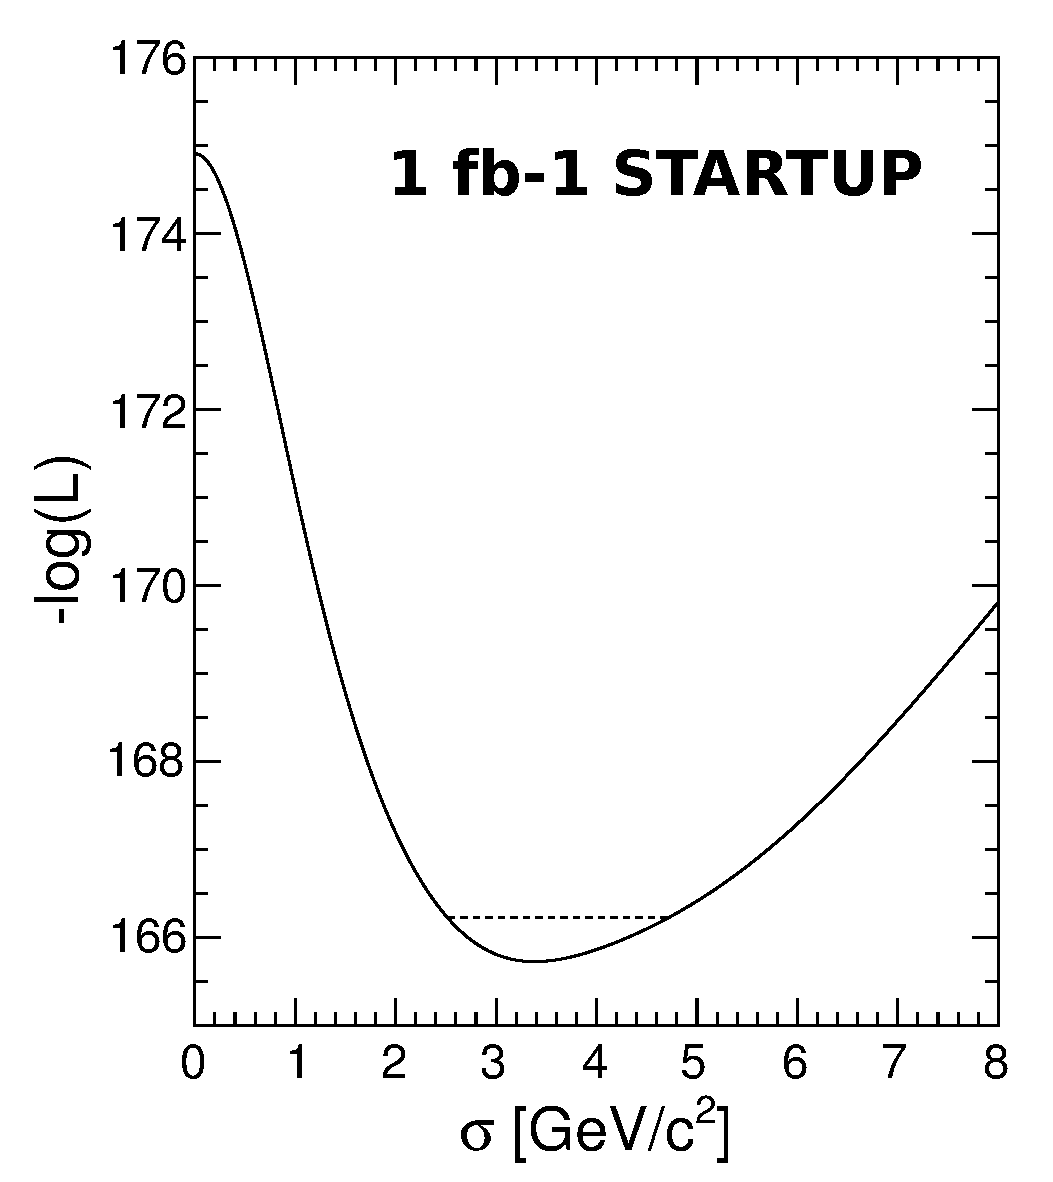
\includegraphics[width=0.49\linewidth]{loglike_startup.pdf}

\column{0.3\linewidth}
\begin{itemize}
\item negligible background from Drell-Yan
\item ansatz simplifies to Voigt with known mass and Lorentzian width
\item only parameter: detector resolution
\item IDEAL: 2.0 $\pm$ 0.6 GeV/$c^2$
\item STARTUP: 3.4 $\pm$ 1.0 GeV/$c^2$
\end{itemize}
\end{columns}
\end{frame}

\begin{frame}
\frametitle{Backup: resolutions from $Z$}
\begin{itemize}
\item Mass resolution ($\sigma_m$) depends primarily on resolution of
  muon momentum magnitudes ($\sigma_{p_1}$ and $\sigma_{p_2}$ for
  leading {\scriptsize (1)} and \mbox{sub-leading {\scriptsize (2)})\hspace{-1 cm}}

\[ {\sigma_m}^2 = {\sigma_{p_1}}^2 \left(\frac{\partial m}{\partial p_1}\right)^2 + 
{\sigma_{p_2}}^2 \left(\frac{\partial m}{\partial p_2}\right)^2 + \mbox{other parameters} \]

\item Best to do deconvolution, but resolution of $p_1$ dominates
  because $\sigma_{p_1} \left|\frac{\partial m}{\partial
    p_1}\right| \gg \sigma_{p_2} \left|\frac{\partial m}{\partial p_2}\right|$
  (because $\sigma_{p_1} \gg \sigma_{p_2}$)
  
\hfill 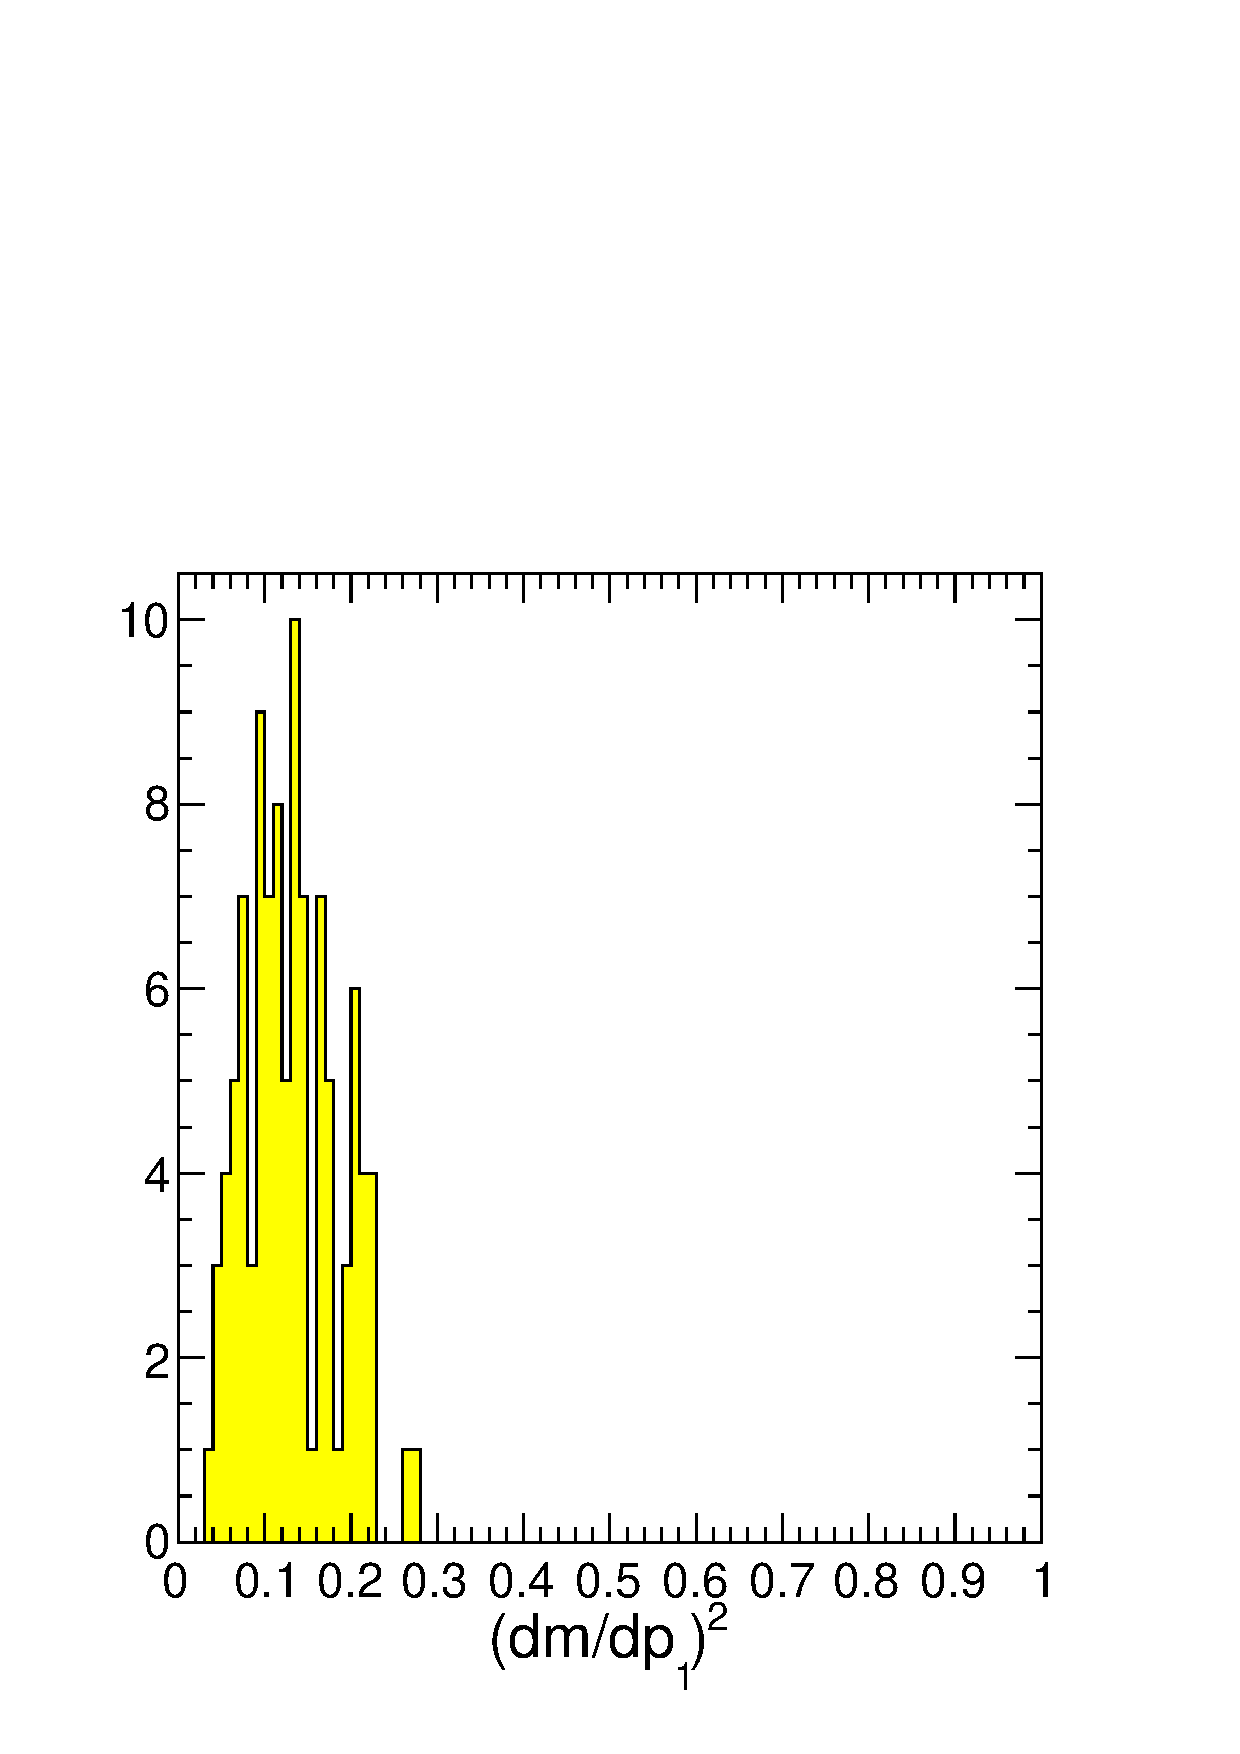
\includegraphics[width=0.3\linewidth]{hist_deriv1_200.pdf}

\vspace{-3.5 cm}
\item $\displaystyle \frac{\partial m}{\partial p_1}$ is 0.05--0.20 (plot on right), so

\renewcommand{\arraystretch}{1.2}
\hspace{0.5 cm}\begin{tabular}{c c}
\scriptsize uncertainty in $\sigma_m$ & \scriptsize uncertainty in $\sigma_{p_1}$ \\\hline
0.6 GeV/$c^2$ & $\sim$4.6 GeV/$c$ \\
1.0 GeV/$c^2$ & $\sim$7.6 GeV/$c$ \\
\end{tabular}

Uncertainty in $\sigma_{p_1}$ is about the same as $\sigma_{p_1}$

\item 1~fb$^{-1}$ is just barely sensitive to $\sigma_{p_1}$ (can be \\ used as a sanity check)
\end{itemize}
\end{frame}

%% mass_200_narrow_linear.pdf
%% mass_200_narrow.pdf
%% 
%% 
%% 
%% hist_derivs_200.pdf
%% 
%% ptone_200.pdf
%% 
%% pttwo_200_linear.pdf
%% pttwo_200.pdf
%% ptone_200_linear.pdf

\end{document}
